\documentclass[conference,a4paper]{IEEEtran}
\IEEEoverridecommandlockouts
\usepackage[utf8]{inputenc}
\usepackage[T1]{fontenc}
\usepackage[english]{babel}
\usepackage{cite}
\usepackage{amsmath,amssymb}
\usepackage{graphicx}
\usepackage{booktabs}
\usepackage{tikz}
\usetikzlibrary{arrows.meta,positioning}
\usepackage[hidelinks]{hyperref}
\usepackage{xurl}
\graphicspath{{figures/}{../../capturas/}}

% Inserts the screenshot if it exists; otherwise draws a labelled placeholder
\newcommand{\captura}[2]{\IfFileExists{capturas/#1}{\includegraphics[width=#2]{capturas/#1}}{\IfFileExists{../../capturas/#1}{\includegraphics[width=#2]{../../capturas/#1}}{\fbox{\parbox[c][2.2cm][c]{0.95#2}{\centering\small Pending screenshot: \detokenize{#1}}}}}}

\begin{document}

\title{Equine Lameness Detection Using Data Mining, Machine Learning and Cloud Computing}

\author{\IEEEauthorblockN{Carlos Josué Barrera Vargas}
\IEEEauthorblockA{Faculty of Data Engineering and Artificial Intelligence\\
Universidad Santo Tomás, Tunja, Colombia\\
Fifth-semester integrative project · Data Mining, Machine Learning and Cloud Computing\\
Repository: \url{https://github.com/Cjoh210/Proyecto_Deteccion_Marcha_Equina}}}

\maketitle

\begin{abstract}
Lameness is the most common health problem in horses, and when it is mild, veterinarians often disagree on the diagnosis. This work builds the foundation of a decision-support system to detect it objectively, which will later work with videos recorded on a phone. Following CRISP-DM, three sources were integrated: a corpus of scientific papers collected from an API, a catalogue of open datasets, and sensor signals from 22 horses with induced lameness. Data mining revealed a field moving towards computer vision, with little research on horses or in Colombia, and no open dataset combining video and lameness. The signals confirmed that asymmetry in head and pelvis movement reveals lameness. An optimized Random Forest validated on unseen horses distinguished it better than chance, and SHAP showed that it relies on the same markers used in clinical practice. The system was deployed on AWS with Terraform, using a serverless architecture that costs cents per month. The project contributes to SDGs 3 and 8.
\end{abstract}

\begin{IEEEkeywords}
data mining, CRISP-DM, ensemble learning, cloud computing, equine lameness, sustainable development
\end{IEEEkeywords}

% =====================================================================
\section{Introduction}
Lameness is the most frequent reason for veterinary consultation in horses and one of the costliest conditions for the sector, due to lost days of use and the treatment it requires~\cite{nehs2013,usda1998}. Its diagnosis relies mainly on watching the animal trot, and several studies show that veterinarians agree poorly with each other when lameness is mild~\cite{keegan2010,hammarberg2016}.

Colombia has close to one million equines~\cite{agronegocios2025censo}, and the Colombian criollo horse has significant cultural and economic value in regions such as Boyacá. A system that estimates lameness from a phone video would make objective assessment available to field veterinarians and breeders. Before building it, this work answers three questions: what has been researched and where the gap is, which public data are available, and which movement signals reveal a lame horse. With those answers, a predictive model was built and deployed in the cloud as a service that works end to end.

% =====================================================================
\section{Problem Statement}
Lameness assessment is subjective, and objective methods, such as body-mounted sensors, force plates or motion capture, are expensive or require instrumenting the animal. This puts them out of reach for many rural breeders and veterinarians.

\textbf{Research question.} Can the probability that a horse is lame be estimated from movement data obtainable with accessible technology, in an interpretable way and at a low deployment cost?

\textbf{Users and beneficiaries.} Field veterinarians, who gain an objective second opinion and follow-up over time; criollo horse breeders and associations, who can monitor their animals; and the horses themselves, which receive an earlier diagnosis.

\textbf{SDG alignment.} The project is linked to SDG 3, Good health and well-being, through the One Health approach that integrates animal and human health~\cite{un2015}, and to SDG 8, Decent work and economic growth, by reducing losses in a rural sector that generates employment.

% =====================================================================
\section{Related Work}
Objective lameness assessment has relied on inertial sensors on the head and pelvis, which measure how uneven the vertical displacement is in each step; these measures correlate with clinical examination, although they do not replace it~\cite{keegan2013}. In computer vision, DeepLabCut made it possible to locate anatomical points in video without markers~\cite{mathis2018}, and horse datasets such as Horse-10 and PFERD followed~\cite{mathis2021,li2024pferd}, along with multi-species pose benchmarks such as AP-10K, APT-36K and Animal Kingdom~\cite{yu2021ap10k,yang2022apt36k,ng2022animalkingdom}. None of them includes clinical lameness labels. Automatic detection is more advanced in cattle, with public databases such as CowScreeningDB~\cite{ismail2024cow}. This work quantifies that gap and proposes a way to close it.

% =====================================================================
\section{Proposed System}
Fig.~\ref{fig:sistema} shows the complete system. The three sources feed a cloud data lake; the data mining pipeline prepares and analyses the data; a model learns to recognize lameness from gait symmetry measures; and an API delivers the predictions and stores them for follow-up. In the computer vision phase, the same measures will be computed from video, so the model and infrastructure built here are reused without changes.

\begin{figure}[t]
\centering
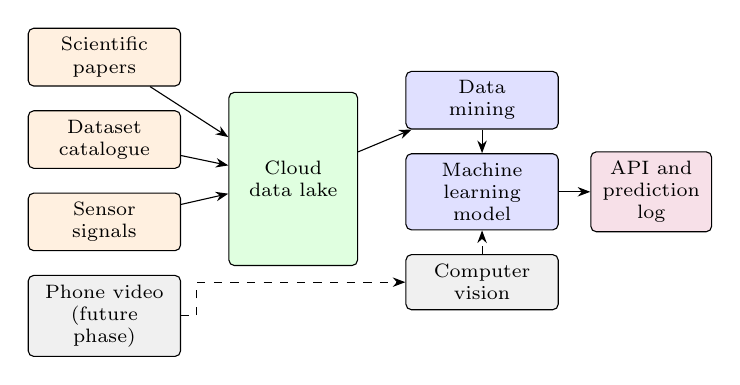
\begin{tikzpicture}[node distance=3mm and 4mm, font=\scriptsize,
  b/.style={draw, rounded corners=2pt, align=center, minimum height=7mm, text width=17mm, fill=#1!12},
  b/.default=blue, >={Stealth[length=1.6mm]}]
\node[b=orange] (api) {Scientific\\papers};
\node[b=orange, below=of api] (cat) {Dataset\\catalogue};
\node[b=orange, below=of cat] (imu) {Sensor\\signals};
\node[b=gray, below=of imu] (vid) {Phone video\\(future phase)};
\node[b=green, right=6mm of cat, yshift=-5mm, text width=14mm, minimum height=22mm] (lake) {Cloud\\data lake};
\node[b, right=6mm of lake, yshift=10mm] (kdd) {Data\\mining};
\node[b, below=of kdd] (ml) {Machine\\learning\\model};
\node[b=gray, below=of ml] (cv) {Computer\\vision};
\node[b=purple, right=4mm of ml, text width=13mm] (srv) {API and\\prediction\\log};
\draw[->] (api) -- (lake); \draw[->] (cat) -- (lake); \draw[->] (imu) -- (lake);
\draw[->, dashed] (vid.east) -- ++(2mm,0) |- (cv.west);
\draw[->] (lake) -- (kdd); \draw[->] (kdd) -- (ml); \draw[->, dashed] (cv) -- (ml); \draw[->] (ml) -- (srv);
\end{tikzpicture}
\caption{General structure of the system. Grey components belong to the computer vision phase.}
\label{fig:sistema}
\end{figure}

% =====================================================================
\section{Data Mining Pipeline}
The process follows the CRISP-DM phases~\cite{wirth2000} and is implemented in six reproducible notebooks.

\subsection{Acquisition}
\textbf{Web scraping of the state of the art.} A Python module queries the OpenAlex API~\cite{priem2022openalex} with five thematic searches: equine lameness, equine gait, sensors, animal vision and pose, and lameness with machine learning in other species. Its role in the system is concrete: to build and keep up to date the knowledge base that justifies the project. It gathered about 6,500 records, and in the cloud it runs every week.

\textbf{Dataset catalogue.} Fourteen public datasets were documented with their characteristics and source link.

\textbf{Sensor signals.} An open dataset was downloaded with 22 Icelandic horses measured while sound and with a mild lameness induced in a fore or hind limb, recorded with sixteen inertial sensors~\cite{smit2023dataset}.

\subsection{Preparation}
In the corpus, papers repeated across searches were merged, non-scientific, retracted or off-topic documents were discarded, and duplicate versions of the same work were unified. A little over four thousand papers remained. Missing abstracts and countries were handled without inventing information: the text was completed with the title and keywords, and unknown country was kept as its own category.

\subsection{Feature Engineering}
The raw sensor signals, on the order of millions of samples, are not useful by themselves. Straight-line trot segments were selected, the vertical displacement of the head, withers, sacrum and hips was computed, and the gait was split into strides. Clinically meaningful measures were extracted from each stride: the difference between the two lowest and the two highest points of each cycle, the range of motion, the regularity of the rhythm and the difference between hips. The result is a table of about 1,800 strides with 27 variables. Missing values from one sensor were imputed with the median of the same horse, and the few physically impossible strides were removed. On this table, PCA showed that several measures are redundant and that sound and lame strides largely overlap, which anticipates the difficulty of the problem (Fig.~\ref{fig:pca}).

\begin{figure}[t]
\centering
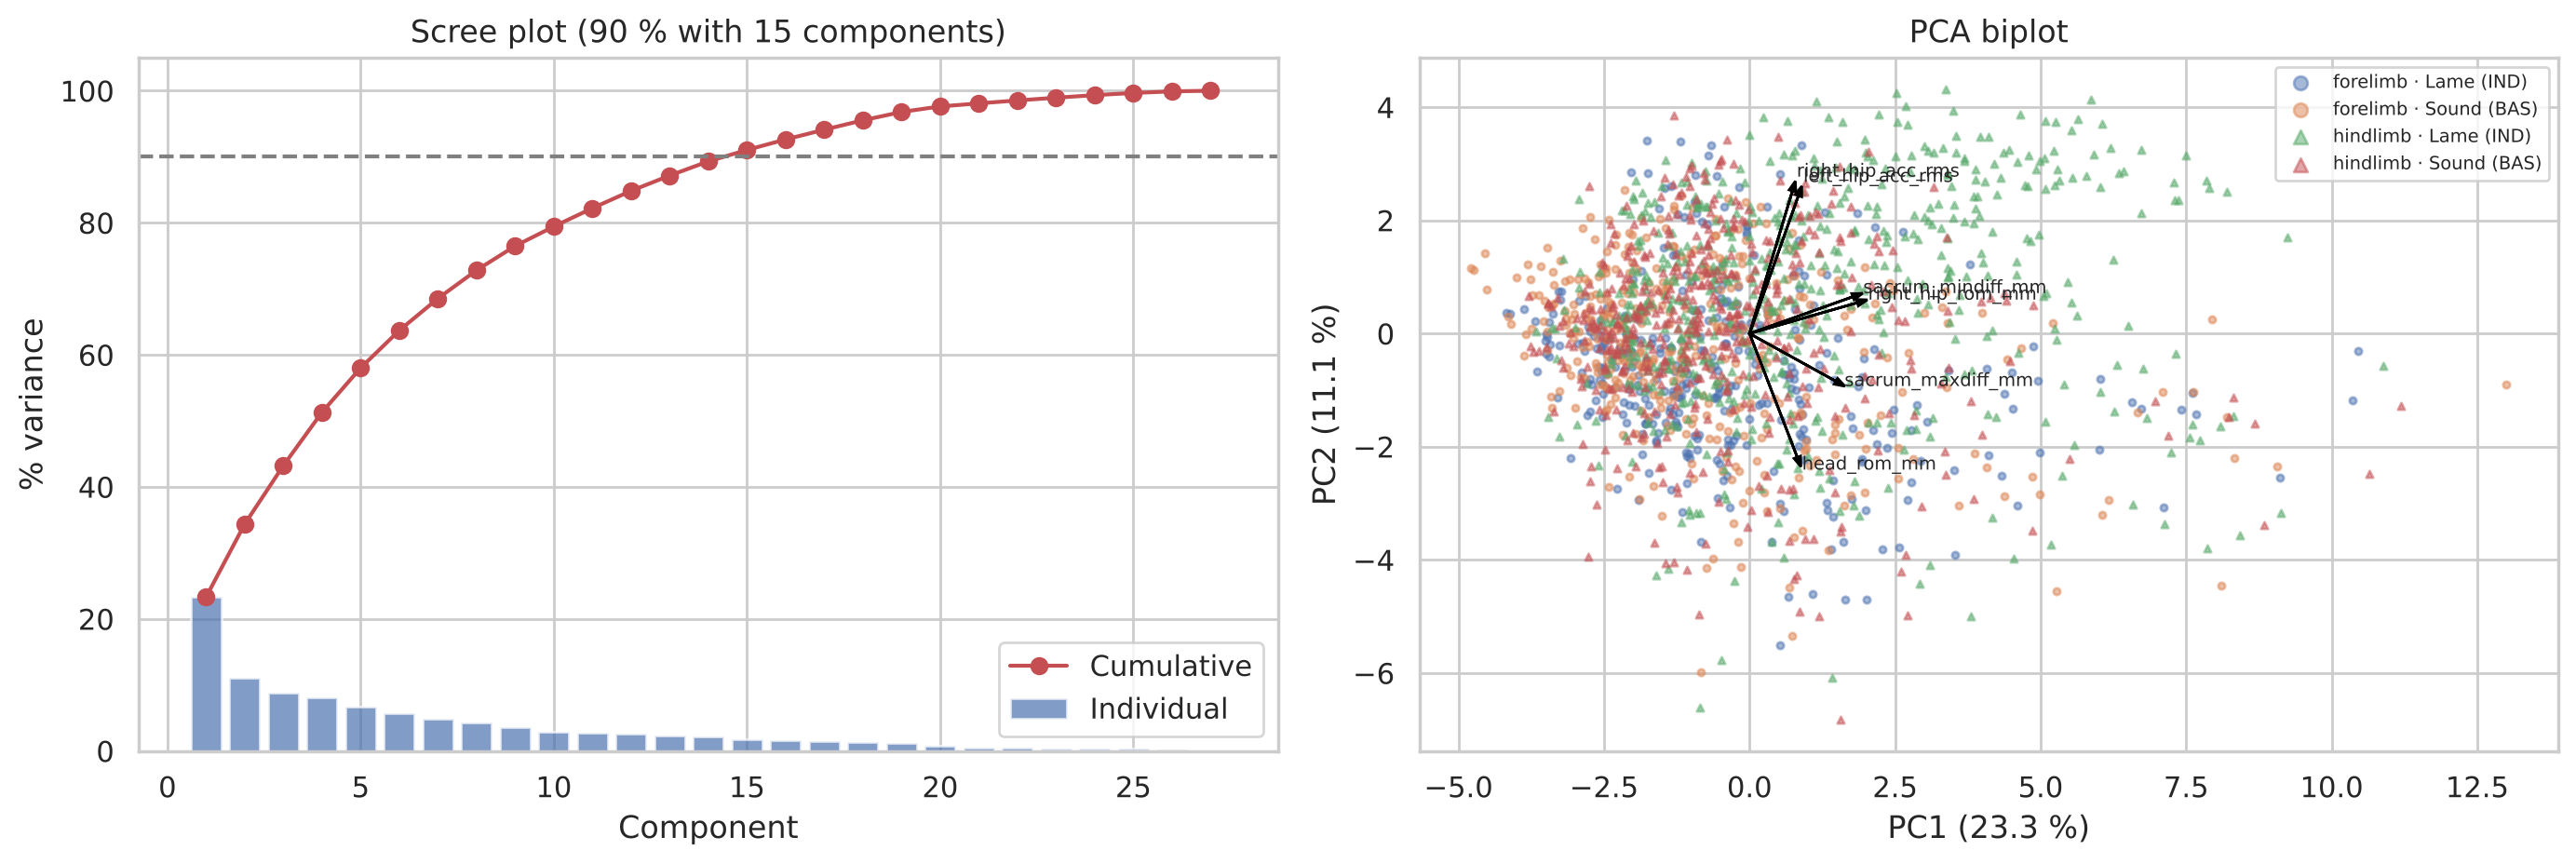
\includegraphics[width=\columnwidth]{imu_pca.png}
\caption{Variance explained by PCA and projection of the strides on the first two components.}
\label{fig:pca}
\end{figure}

\subsection{Exploratory Analysis and Outliers}
The corpus EDA described the evolution over time, countries, journals and impact of the papers. For the sensors, each horse was compared with itself before and after induction using the paired Wilcoxon test, which respects the fact that strides from the same animal are not independent.

Outliers were interpreted before deciding what to do with them. In the corpus, papers with exceptional impact turned out to be the most widely used computer vision tools in the field, its technological frontier, so they were kept. In the sensors, Isolation Forest showed that anomalous strides concentrate in lame horses: much of the anomaly is the clinical signal itself. Only impossible records and real noise were removed, such as studies on equine semen that the search had brought in by mistake.

\subsection{Unsupervised Mining}
The corpus texts were represented with TF-IDF, reduced with SVD and grouped with K-Means, choosing the number of groups with four internal metrics and comparing the result with hierarchical clustering and DBSCAN (Fig.~\ref{fig:k}). DBSCAN was discarded because it labelled almost half of the papers as noise. Keywords were analysed with association rules using Apriori and FP-Growth~\cite{agrawal1994,han2000}, which found the same frequent itemsets.

\begin{figure}[t]
\centering
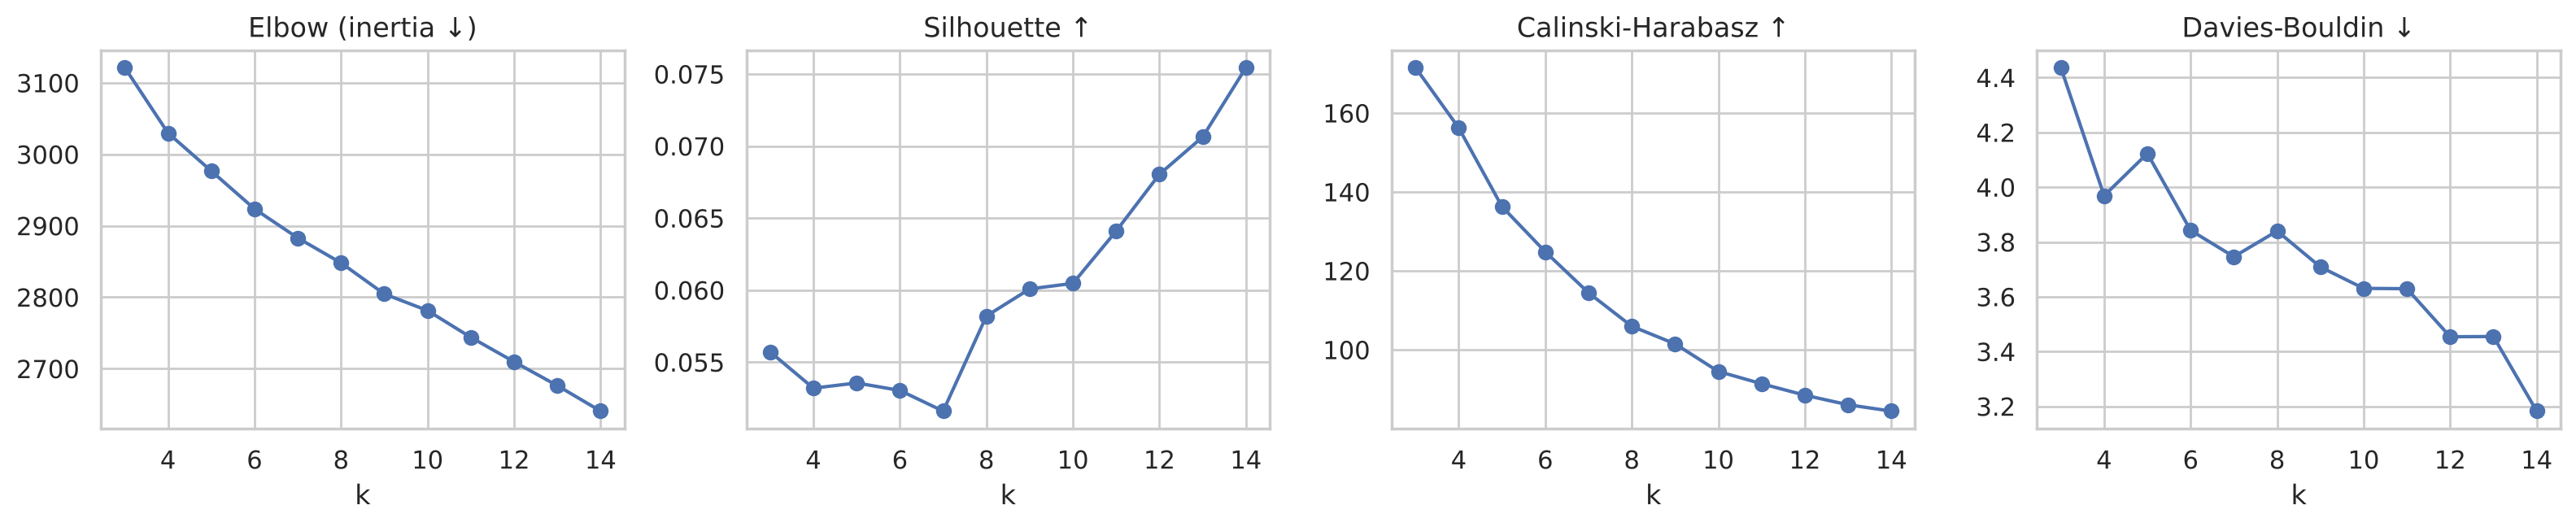
\includegraphics[width=\columnwidth]{art_kmeans_seleccion_k.png}
\caption{Metrics used to choose the number of K-Means clusters.}
\label{fig:k}
\end{figure}

The catalogue was clustered hierarchically with the Gower distance, which suits mixed variables, and the strides were grouped with K-Means and hierarchical clustering to identify movement and horse profiles.

% =====================================================================
\section{Machine Learning Models}
\subsection{Lameness Classifier}
The main model classifies each stride as sound or lame. The central methodological decision was to \emph{always validate on horses the model has not seen}: strides from the same animal are so similar that mixing them between training and test would make the model recognize the horse rather than the lameness. Therefore, five complete horses were held out for the final test, model selection used cross-validation grouped by horse, and robustness was checked by leaving one horse out at a time.

All models share a pipeline of imputation, scaling and classification, fitted inside each fold to avoid data leakage. Logistic regression, KNN and SVM were compared with the Random Forest, AdaBoost and Gradient Boosting ensembles~\cite{breiman2001}. Hyperparameters were optimized with Grid Search for Random Forest and Gradient Boosting, and with Random Search for SVM. The final model was interpreted with SHAP~\cite{lundberg2017}.

\subsection{Regression of Scientific Impact}
As a complement, the impact of the papers, measured as citations per year, was modelled from their characteristics: topic, document type, collaboration, open access and thematic profile. Linear, polynomial, Ridge, Lasso and Elastic Net regression were compared~\cite{tibshirani1996,zou2005}, with Grid Search over the regularization strength, and a Random Forest as reference. The goal was not to predict citations, but to understand which kind of work is most influential in the field.

% =====================================================================
\section{Cloud Architecture}
\subsection{Selection and Justification}
AWS was chosen in a public cloud deployment, for its maturity, documentation and free tier. The service model is mainly \emph{FaaS} and \emph{PaaS}: Lambda functions and managed services instead of virtual servers. The reason is the nature of the workload, which is intermittent: a weekly ingestion and occasional predictions. An EC2 server would be billed 24 hours a day even if nobody used it, whereas the serverless design only incurs cost when it works. For the same reason, on-demand DynamoDB was chosen instead of an always-on relational database.

\subsection{Components}
The architecture in Fig.~\ref{fig:aws} has four blocks. In \emph{ingestion}, EventBridge triggers a weekly Lambda that runs the web scraping, with the API key stored encrypted in Parameter Store. The \emph{data lake} in S3 is organized into raw, processed and model zones, with encryption, versioning and a lifecycle that archives old data. \emph{Analytics} uses Glue and Athena to query the data with SQL directly on S3. \emph{Inference} exposes an HTTP API that invokes a Lambda packaged as a Docker image with scikit-learn; it loads the model from S3 and records each prediction in DynamoDB, which makes it possible to follow each horse over time. CloudWatch, email alerts and a monthly budget monitor errors and costs.

\begin{figure}[t]
\centering
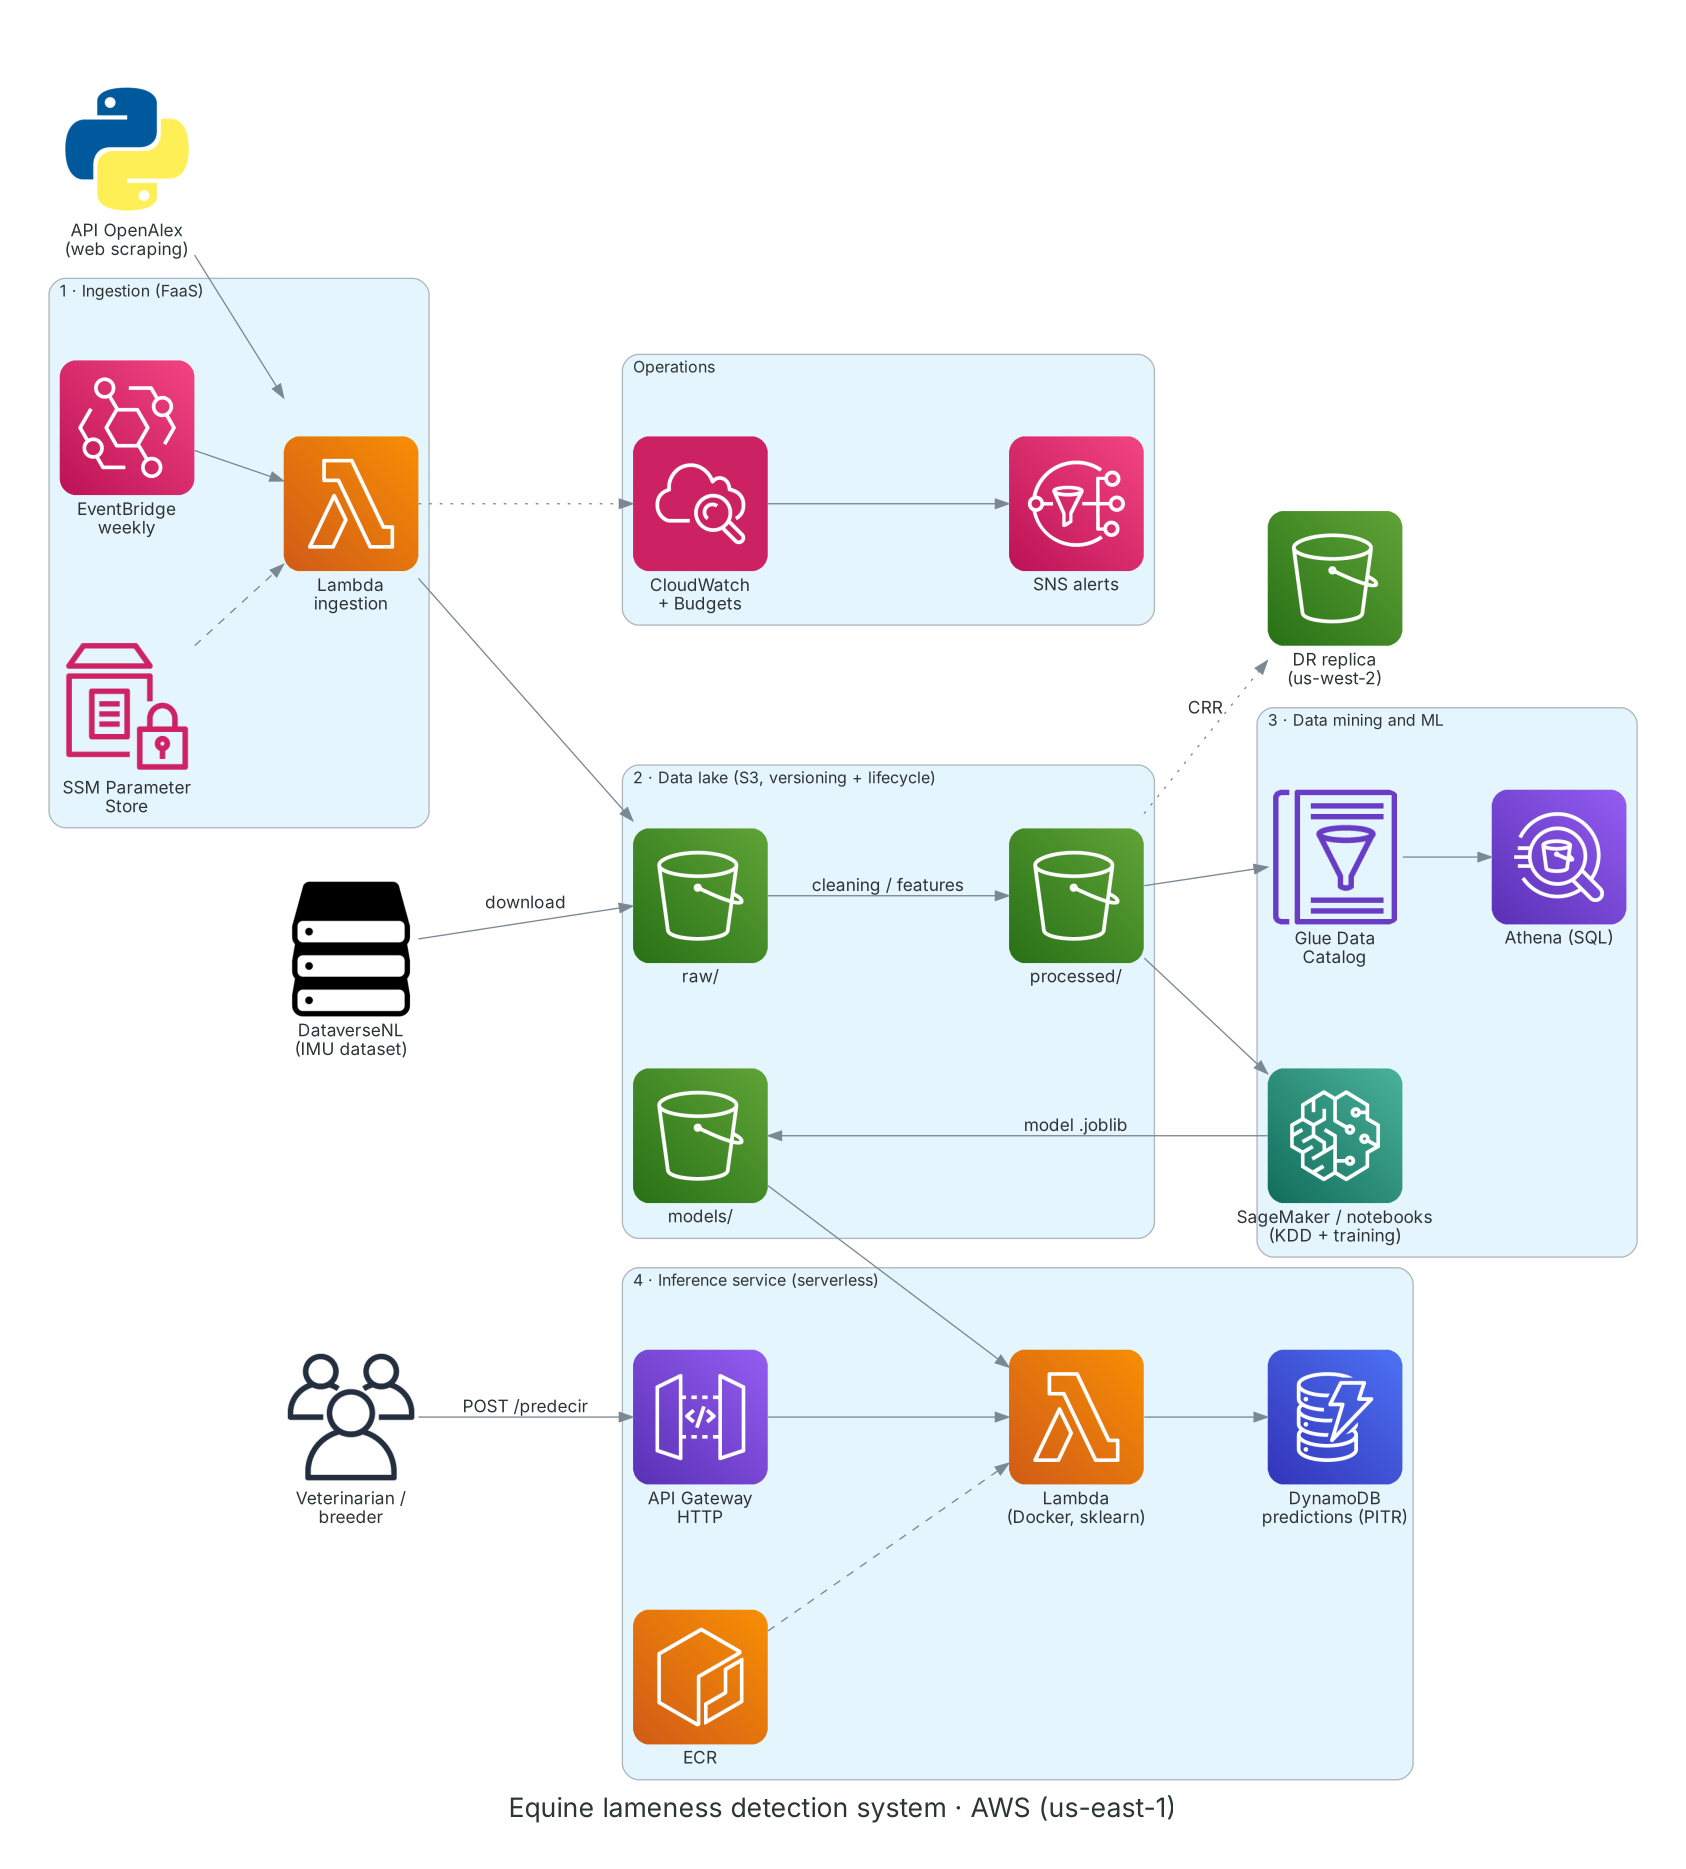
\includegraphics[width=\columnwidth]{arquitectura_aws.png}
\caption{System architecture on AWS.}
\label{fig:aws}
\end{figure}

\subsection{Scalability, Availability and Recovery}
Lambda, API Gateway, S3 and DynamoDB scale automatically with demand and run across several availability zones, so they fulfil the role of auto-scaling and load balancing without manual configuration. The API limits requests per second to protect costs. For disaster recovery, S3 keeps versions of every file, DynamoDB can restore the table to any point in the last 35 days, and an optional replica of the data exists in another region. Since the whole infrastructure is written as code, it can be recreated in minutes.

\subsection{Infrastructure as Code and Deployment}
The infrastructure was written in Terraform~\cite{terraform}, with least-privilege permissions for each component and tags that attribute costs to the project. It was deployed on a real AWS account (Fig.~\ref{fig:apply}). The ingestion function ran in the cloud and stored the same corpus obtained locally (Fig.~\ref{fig:ingesta}). In its first run the function ran out of memory; this was fixed by writing results to disk incrementally. The incident shows the value of testing the deployed system and not only the code.

\begin{figure}[t]
\centering
\captura{terraform_apply.png}{\columnwidth}
\caption{Infrastructure deployment with Terraform.}
\label{fig:apply}
\end{figure}

\begin{figure}[t]
\centering
\captura{s3_openalex.png}{\columnwidth}\\[2mm]
\captura{athena_consulta.png}{\columnwidth}
\caption{Corpus stored in S3 by the weekly ingestion and SQL query in Athena on the sensor data.}
\label{fig:ingesta}
\end{figure}

\subsection{End-to-End Integration}
Fig.~\ref{fig:api} shows the complete system at work: a request with the measures of five strides of a horse reaches the API, the inference Lambda applies the model and returns the probability of lameness, and the prediction is stored in DynamoDB. This is the flow presented in the live demonstration.

\begin{figure}[t]
\centering
\captura{api_respuesta.png}{\columnwidth}\\[2mm]
\captura{dynamodb_items.png}{\columnwidth}
\caption{Inference API response and prediction stored in DynamoDB.}
\label{fig:api}
\end{figure}

% =====================================================================
\section{Results}
\subsection{State of the Art}
Scientific output grows steadily and, in recent years, computer vision has become the dominant approach over traditional clinical studies (Fig.~\ref{fig:tendencia}). Clustering identified eight research lines that separate an older clinical block from a more recent and higher-impact technological block, made up of pose estimation, vision, sensors and detection in cattle (Fig.~\ref{fig:tsne}). Association rules showed that animal pose methods inherit from human pose, and that automatic lameness detection has been developed mainly in dairy cows. The gap is clear: among the works that combine horse, lameness and computer vision, only one has authors in Colombia.

\begin{figure}[t]
\centering
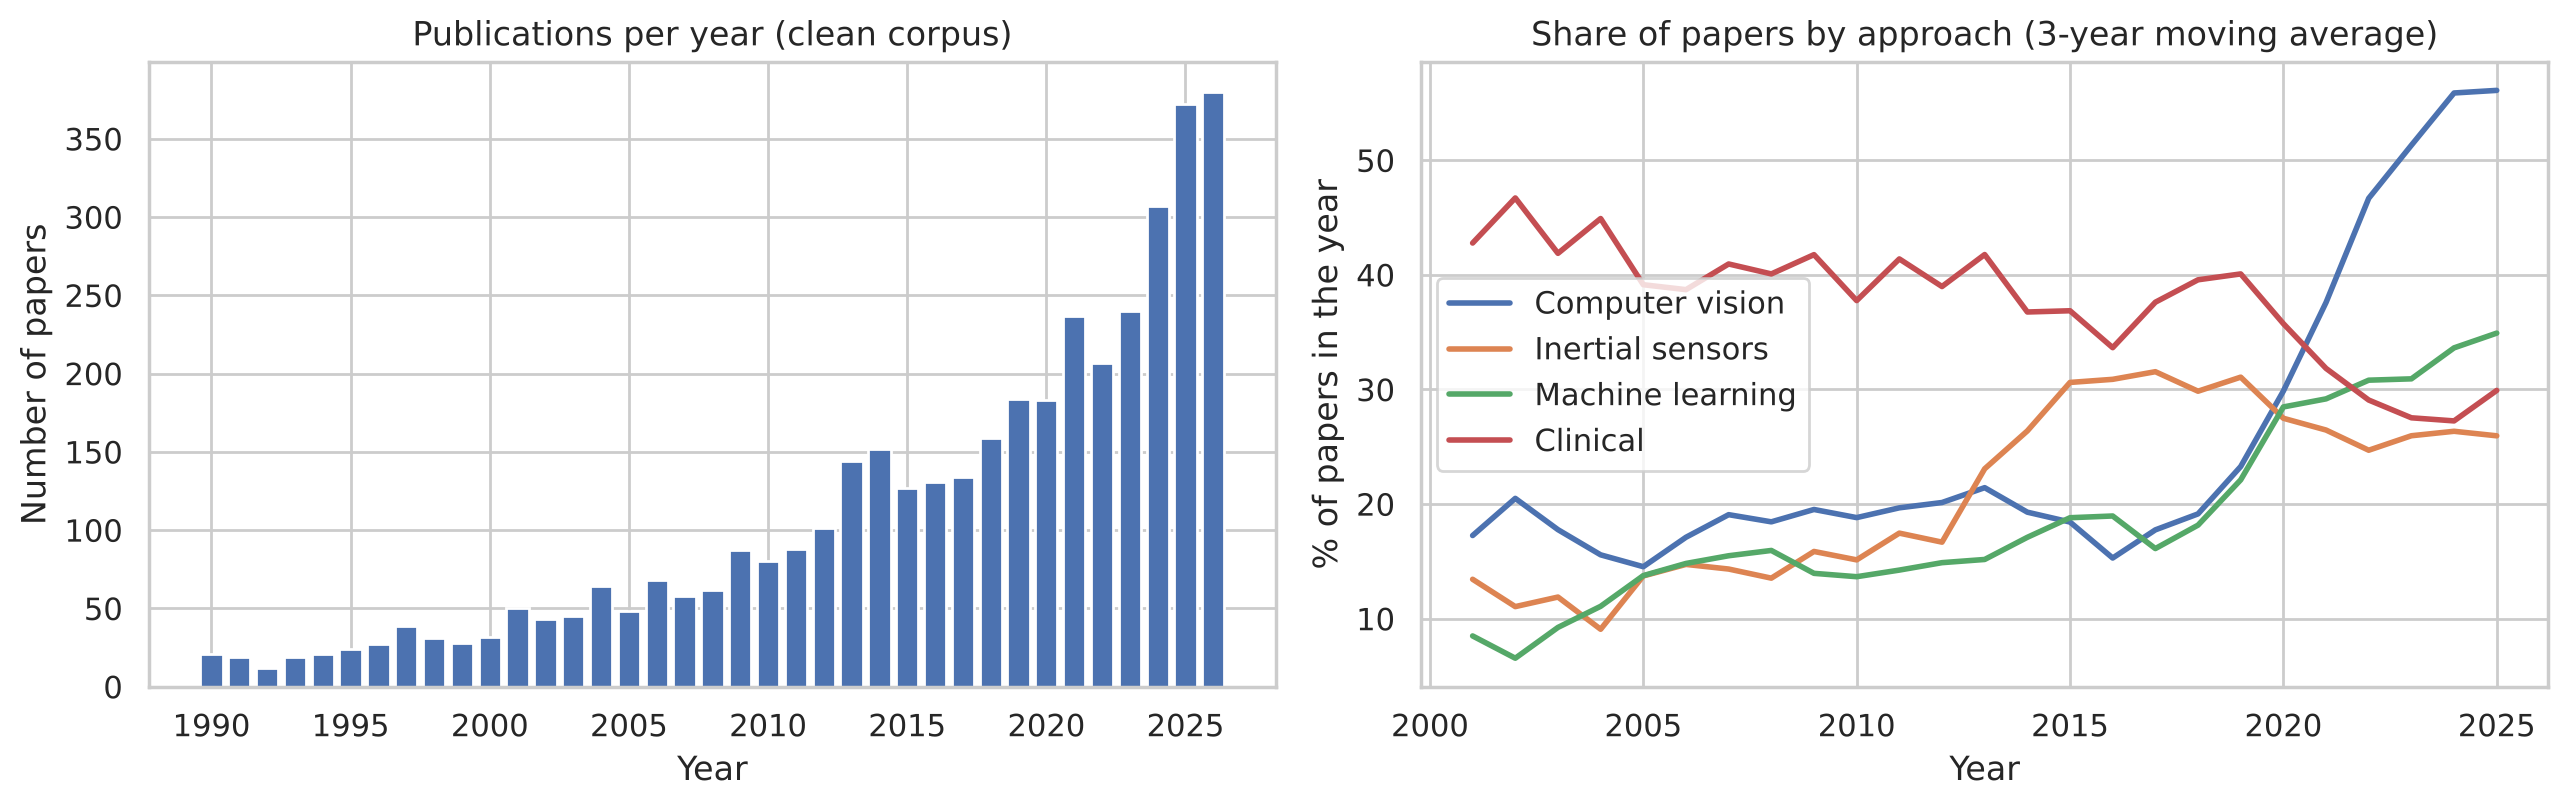
\includegraphics[width=\columnwidth]{art_tendencia_anual.png}
\caption{Publications per year and share of papers by approach. The year 2026 is incomplete.}
\label{fig:tendencia}
\end{figure}

\begin{figure}[t]
\centering
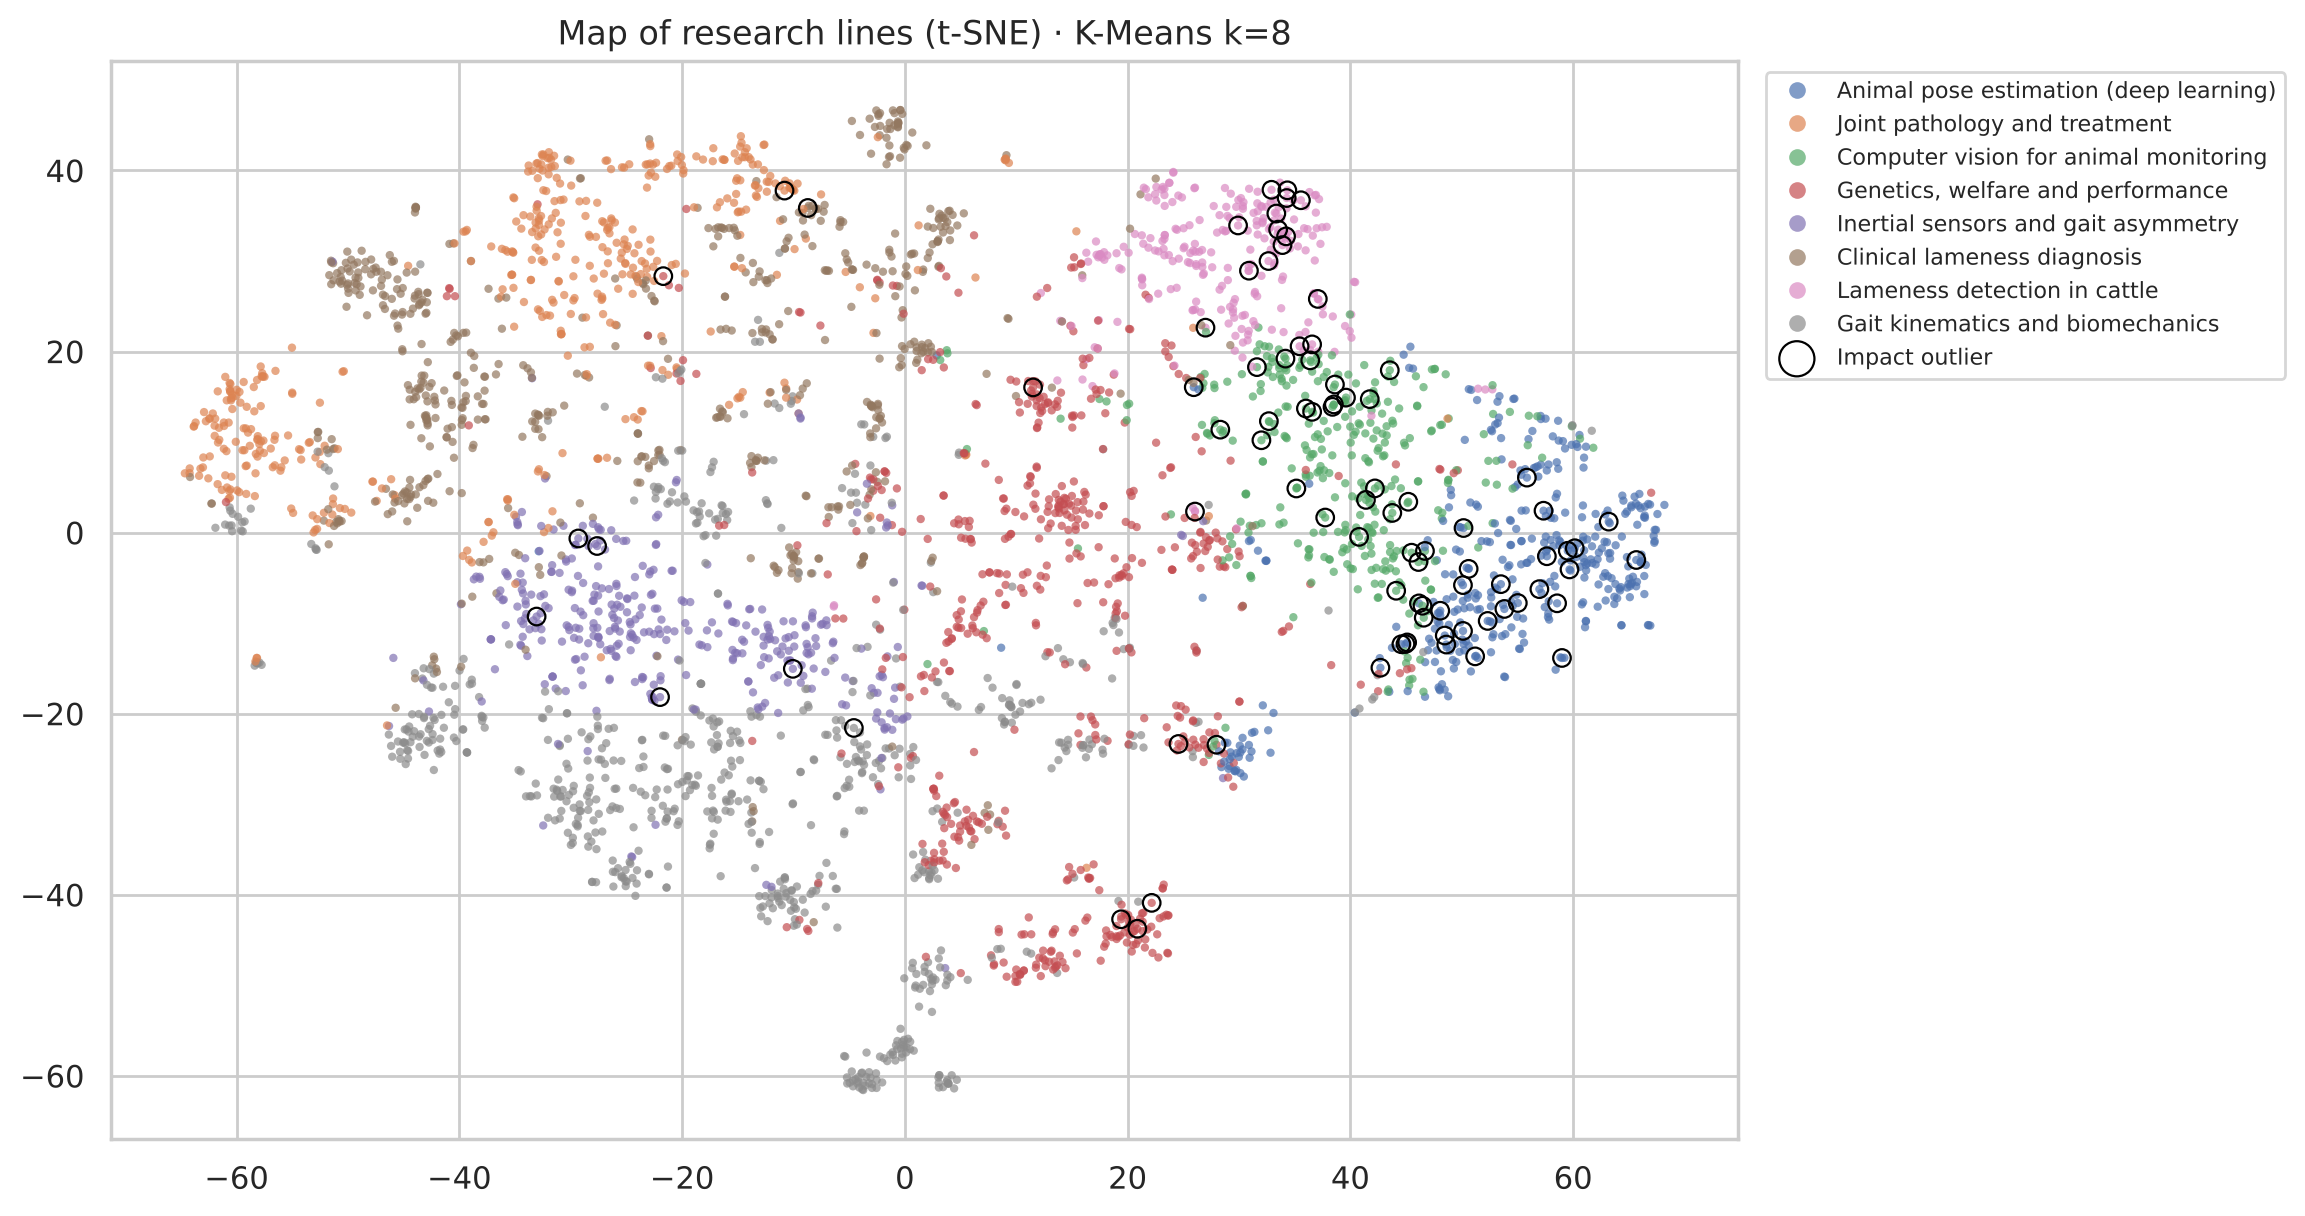
\includegraphics[width=\columnwidth]{art_tsne_clusters.png}
\caption{Map of the research lines found by clustering. Black circles mark papers with outlying impact.}
\label{fig:tsne}
\end{figure}

\subsection{Available Datasets}
The catalogue was organized into four profiles: horse motion capture, sensors with lameness labels, pose images and videos with anatomical keypoints. No public dataset combines horse video with lameness labels (Fig.~\ref{fig:aptitud}). This defines the strategy for the vision phase: learn to locate anatomical points with Horse-10 or AP-10K, check the trajectories against PFERD motion capture, and apply the classifier from this work.

\begin{figure}[t]
\centering
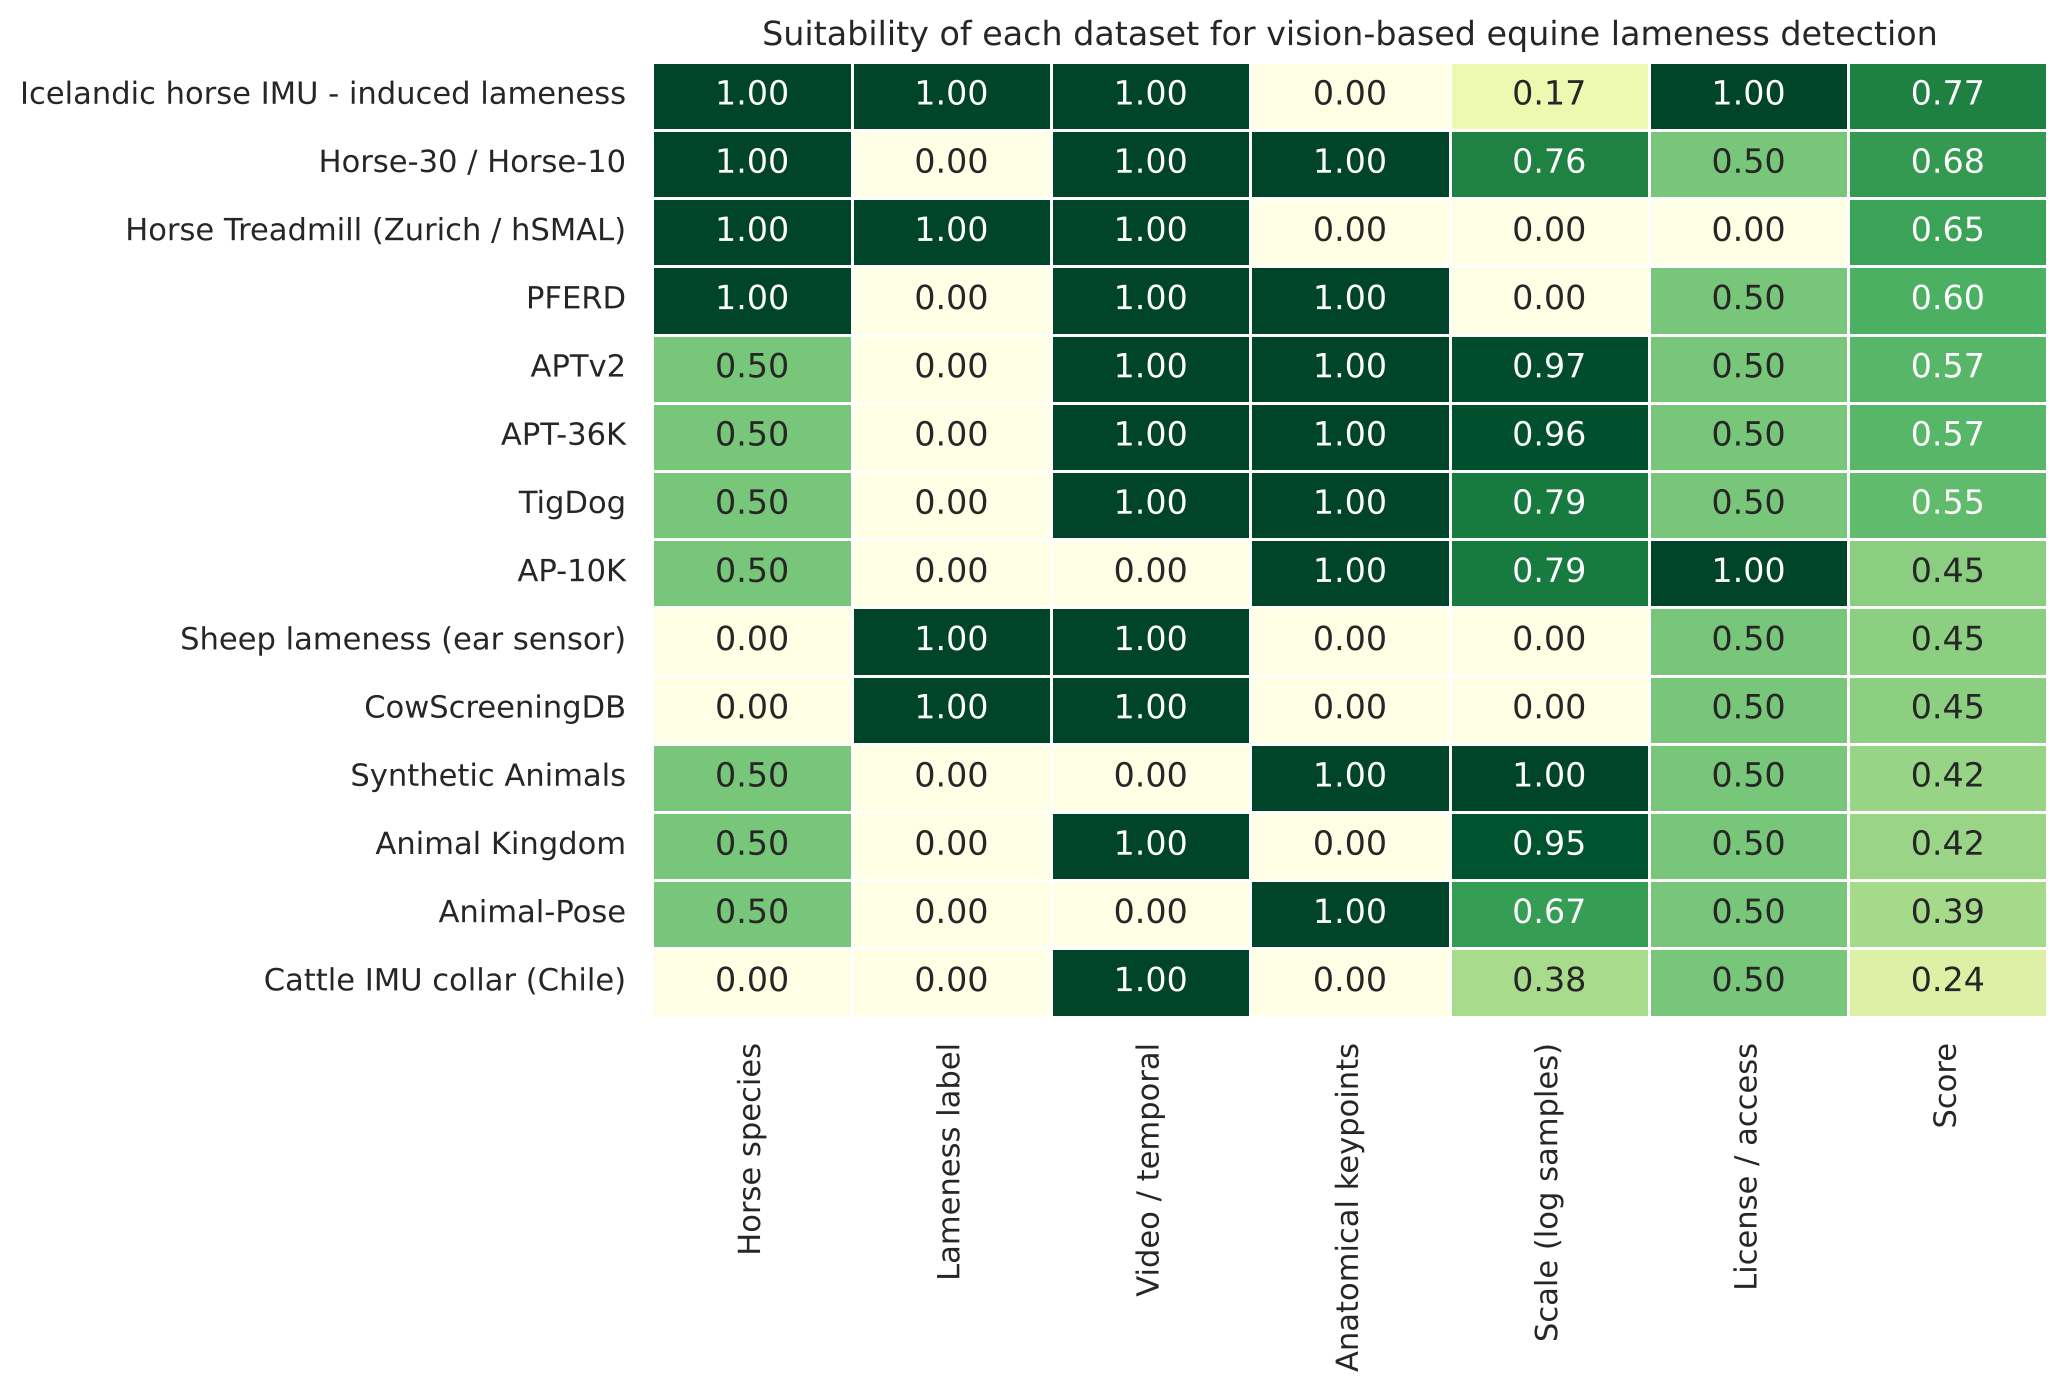
\includegraphics[width=0.9\columnwidth]{cat_matriz_aptitud.png}
\caption{Suitability of each public dataset for the goal of the project.}
\label{fig:aptitud}
\end{figure}

\subsection{Gait Signals}
When each horse was compared with itself, forelimb lameness almost doubled head asymmetry, while hindlimb lameness increased sacrum asymmetry and the difference between hips, with statistically significant differences (Figs.~\ref{fig:pareado} and~\ref{fig:box}). This is the pattern described in clinical practice: the horse lifts its head when it loads a painful front leg, and its hip when the pain is behind. The response varies between individuals, and some horses are asymmetric even when sound. Clustering of horses confirmed it: it largely separated sound from lame horses, except precisely for those individuals. A fixed threshold is therefore not enough.

\begin{figure}[t]
\centering
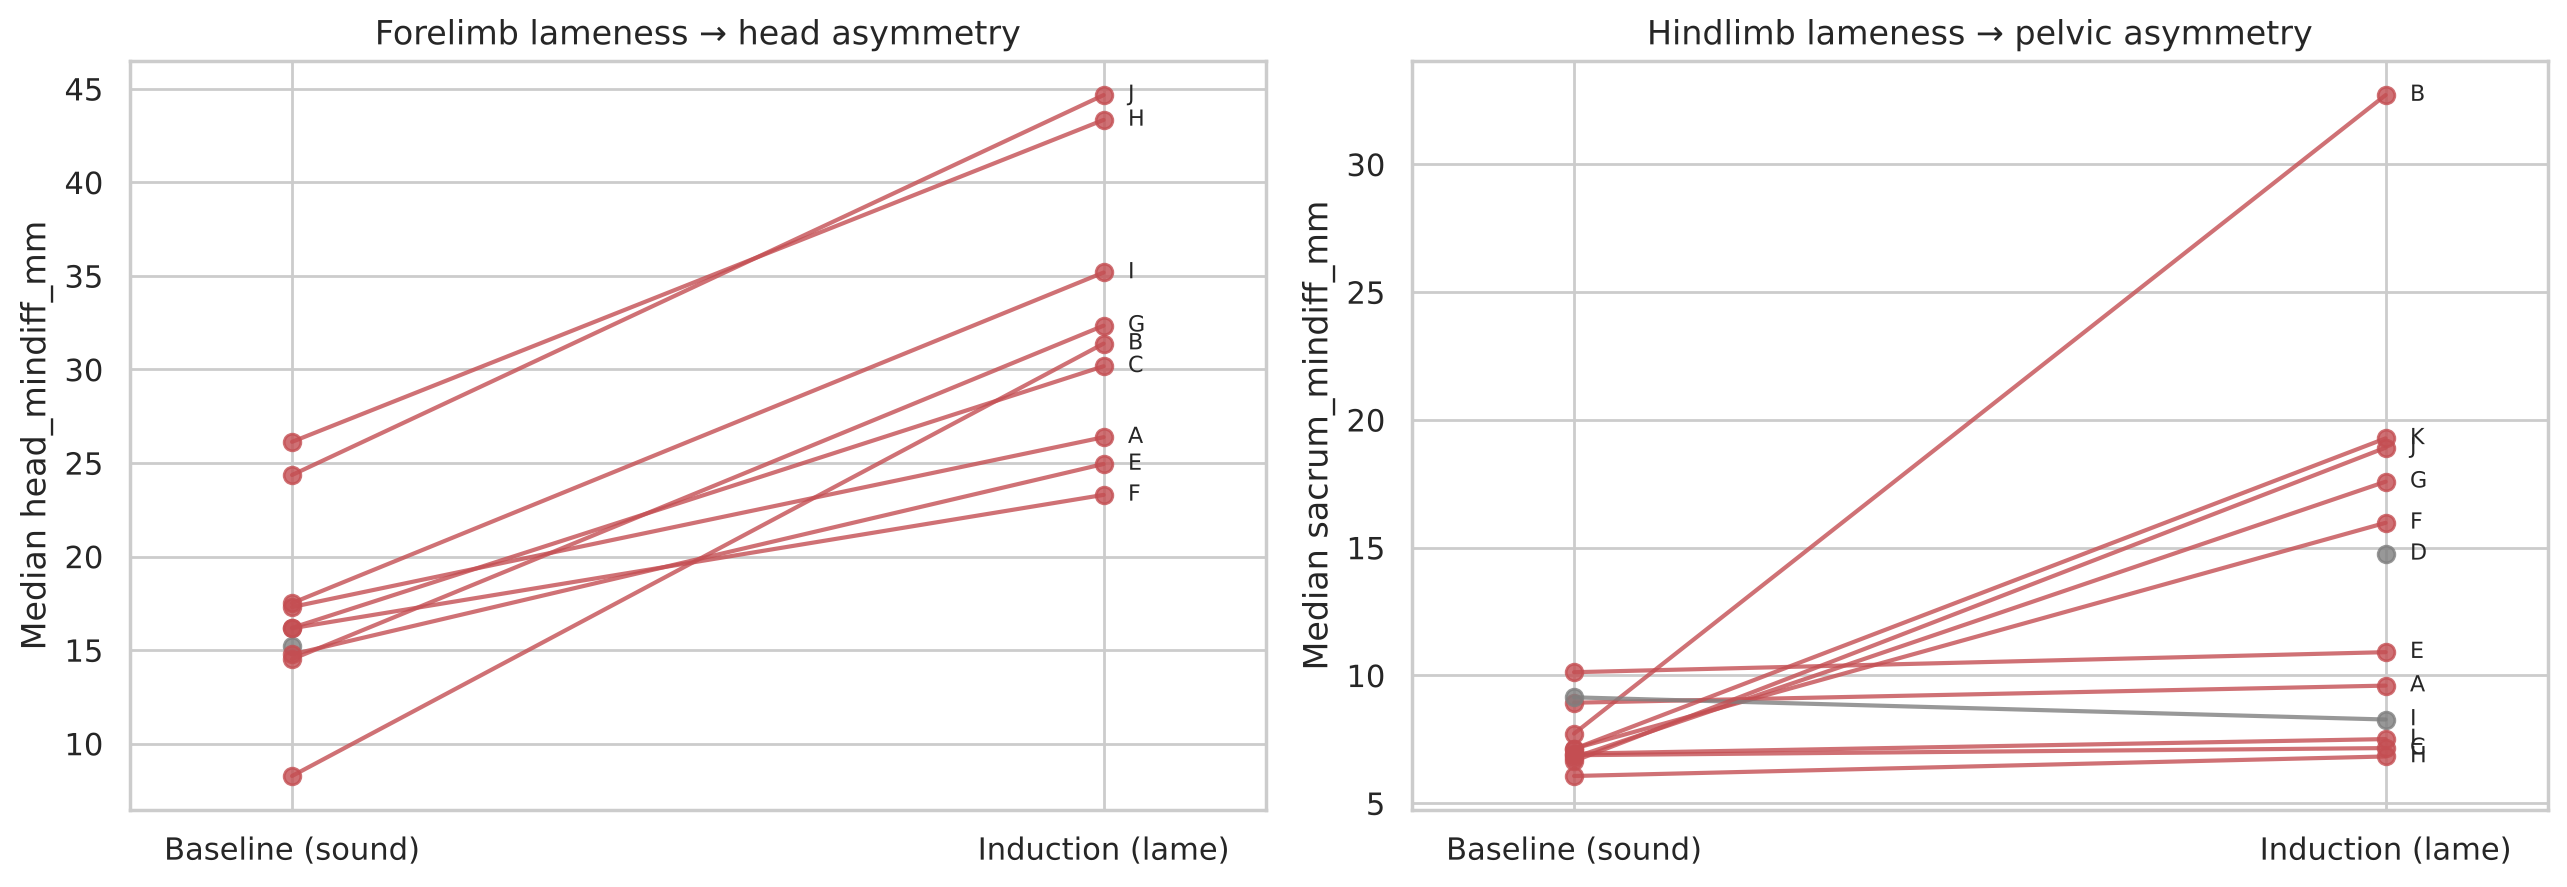
\includegraphics[width=\columnwidth]{imu_pareado_caballos.png}
\caption{Change in each horse's asymmetry between the sound condition and induced lameness.}
\label{fig:pareado}
\end{figure}

\begin{figure*}[t]
\centering
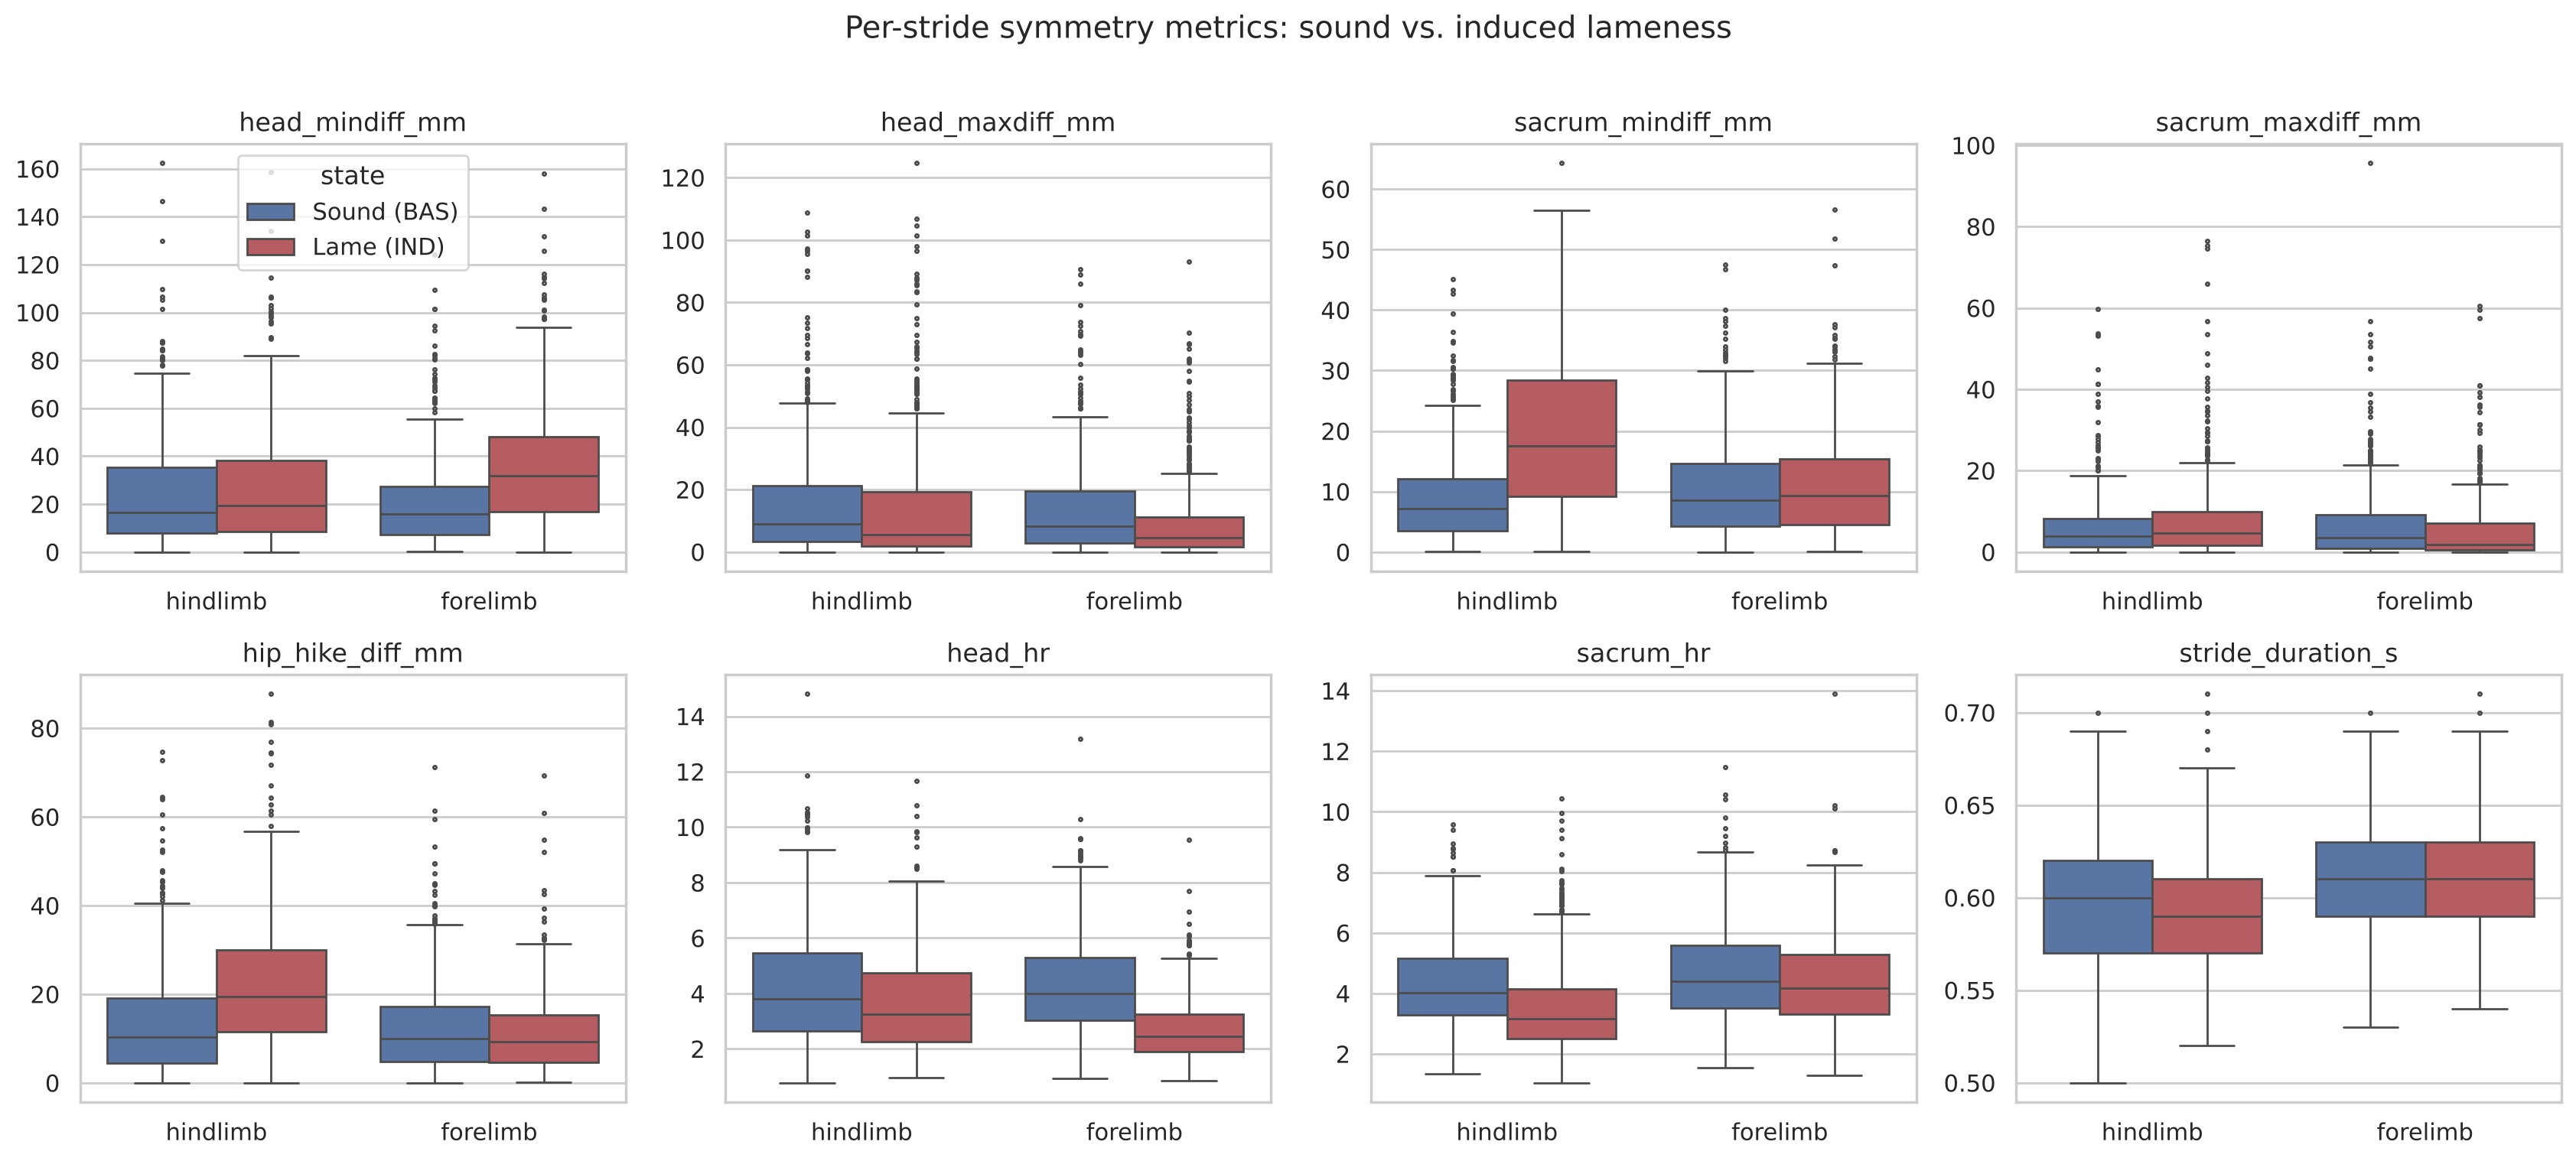
\includegraphics[width=0.85\textwidth]{imu_boxplots.png}
\caption{Distribution of per-stride symmetry metrics in sound horses and horses with induced lameness, by type of lameness.}
\label{fig:box}
\end{figure*}

\subsection{Lameness Classifier}
Table~\ref{tab:ml} summarizes the results. In cross-validation the models were close to each other, and Random Forest was the best ensemble after optimization, so it was chosen as the final model for its performance, its exact interpretability with SHAP and its low computational cost. On the five test horses it reached a ROC-AUC of 0.71, the same value obtained when leaving one horse out at a time, and when averaging the strides of each trot trial it was right in seven out of nine (Fig.~\ref{fig:roc}). Gradient Boosting performed slightly better on the test set, but it was not chosen, because the model is selected through validation and not by looking at the test set. SHAP shows that the model relies on sacrum asymmetry, the regularity of head movement and the difference between hips, the same markers a veterinarian uses (Fig.~\ref{fig:shap}). Performance is moderate, as expected for mild lameness evaluated on new horses, and it is an honest estimate of how the system would work in practice.

\begin{table}[t]
\centering
\caption{Classification with horse-grouped validation (ROC-AUC)}
\label{tab:ml}
\begin{tabular}{lcc}
\toprule
Model & Cross-validation & Test \\
\midrule
Logistic regression & 0.67 & 0.68 \\
Optimized SVM & 0.68 & 0.69 \\
Optimized Gradient Boosting & 0.63 & 0.72 \\
\textbf{Optimized Random Forest} & \textbf{0.67} & \textbf{0.71} \\
\bottomrule
\end{tabular}
\end{table}

\begin{figure}[t]
\centering
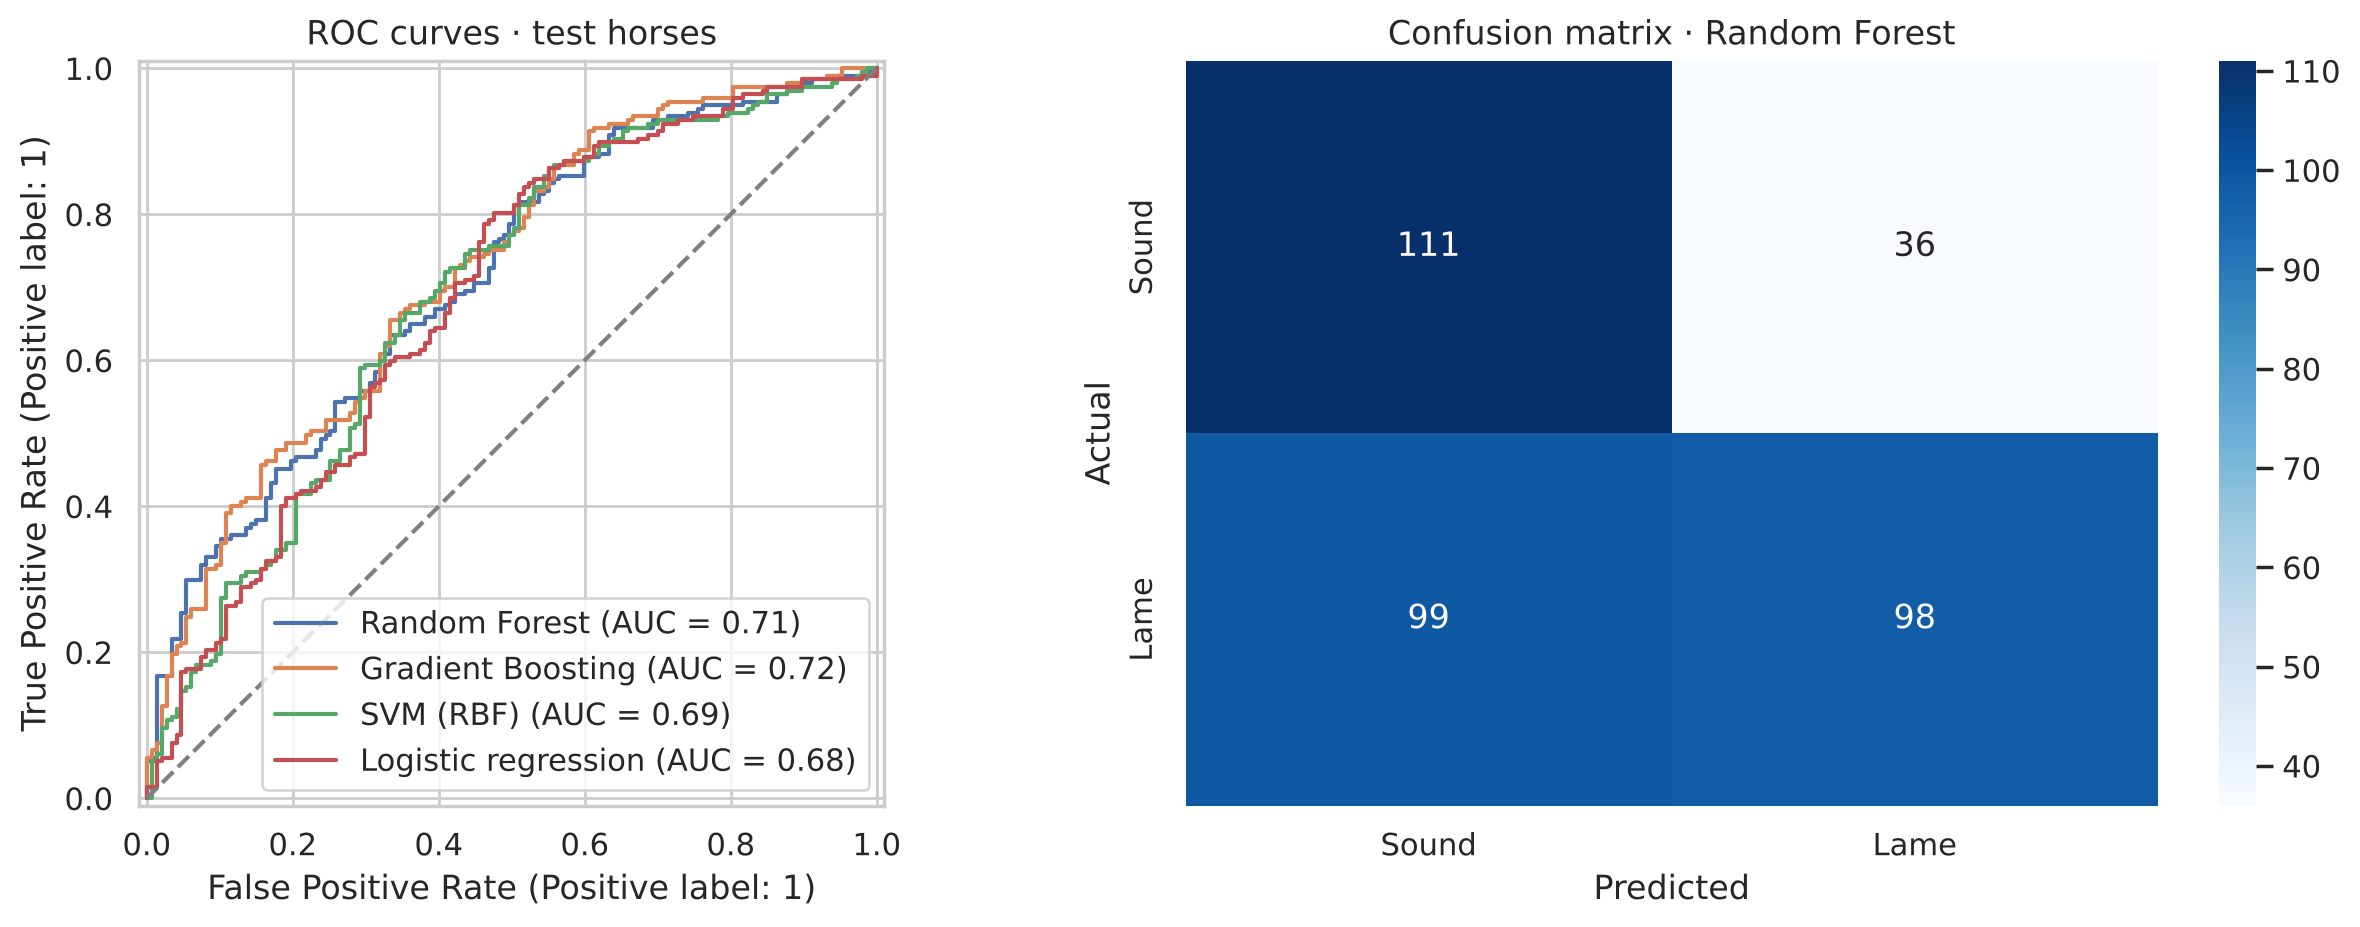
\includegraphics[width=\columnwidth]{ml_roc_confusion.png}
\caption{ROC curves on the test horses and confusion matrix of the final model.}
\label{fig:roc}
\end{figure}

\begin{figure}[t]
\centering
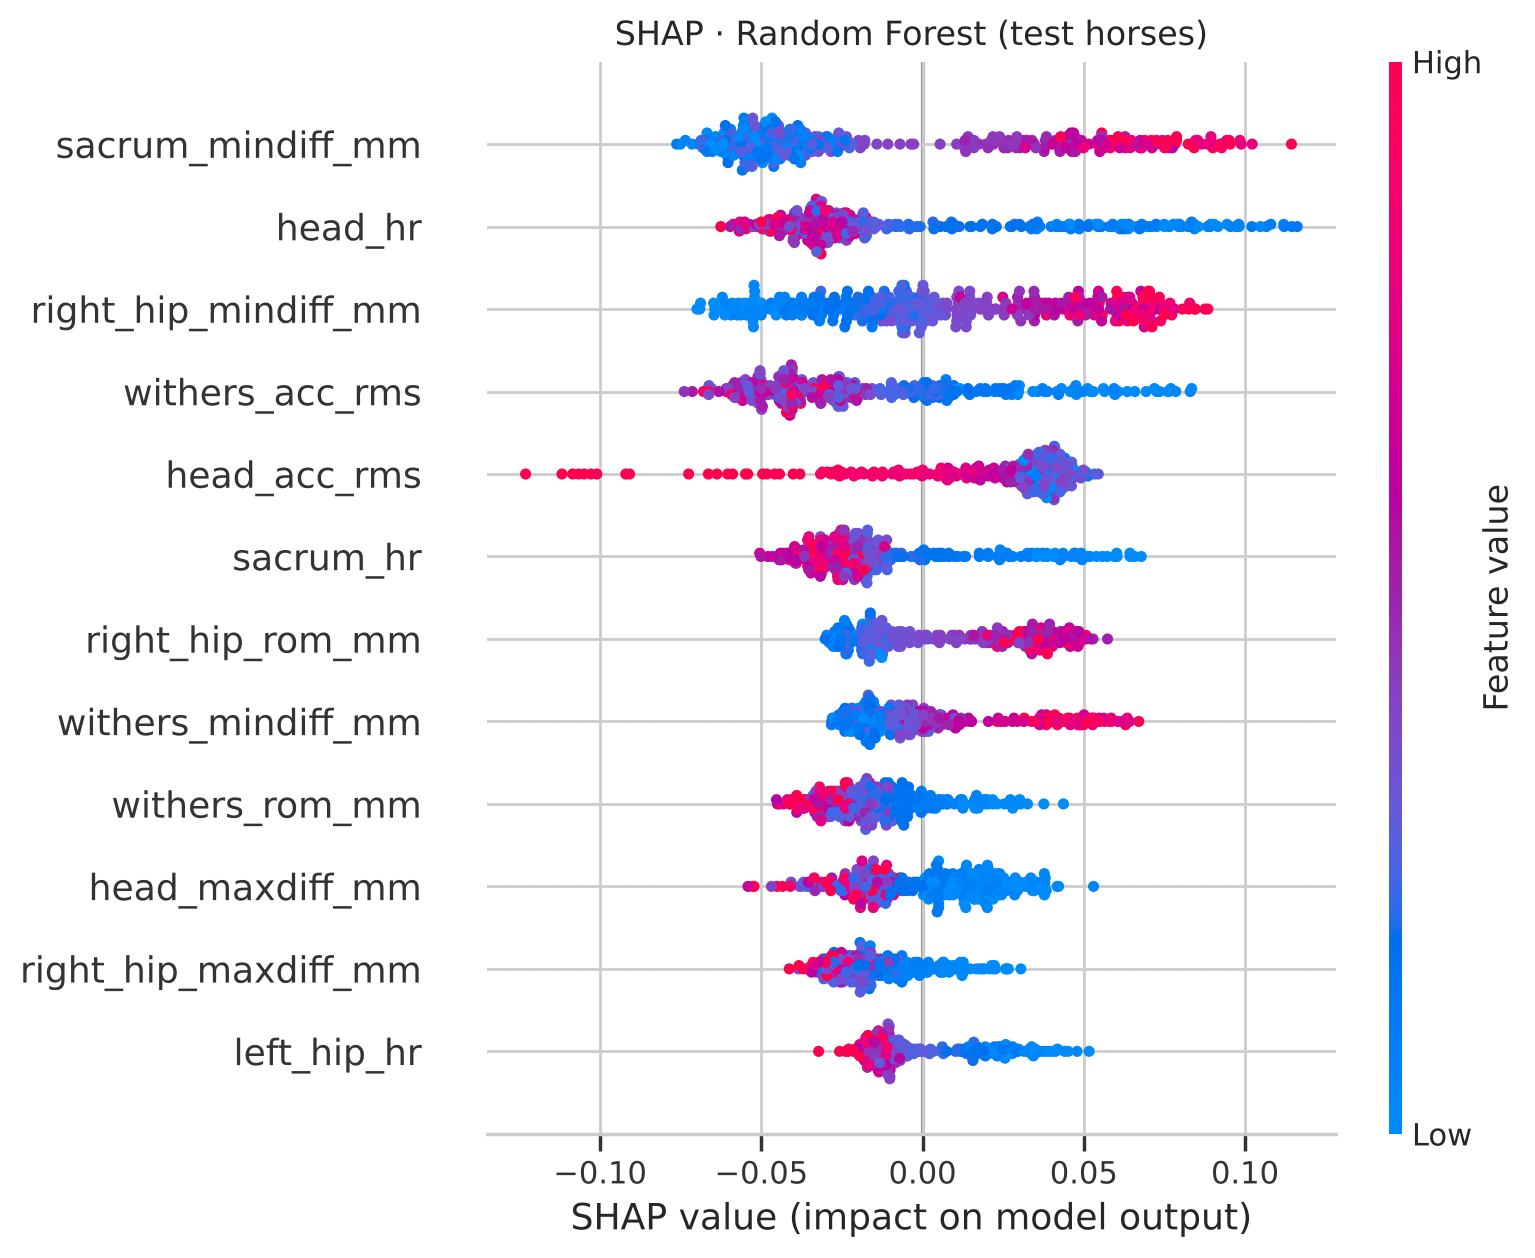
\includegraphics[width=0.85\columnwidth]{ml_shap_summary.png}
\caption{Most influential variables in the model according to SHAP.}
\label{fig:shap}
\end{figure}

\subsection{Scientific Impact}
Linear models explained about 40\,\% of the variation in impact, regularized polynomial regression around 50\,\%, and Random Forest somewhat more, thanks to its ability to capture interactions (Fig.~\ref{fig:reg}). Ridge, Lasso and Elastic Net performed the same as linear regression, because with three thousand papers and few variables there was no overfitting to correct. Their main use was variable selection. Lasso showed that the pose estimation, vision and cattle detection profiles, together with international collaboration, are associated with more citations per year, while the classic clinical profiles are associated with fewer (Fig.~\ref{fig:lasso}). This supports the decision to steer the project towards computer vision.

\begin{figure}[t]
\centering
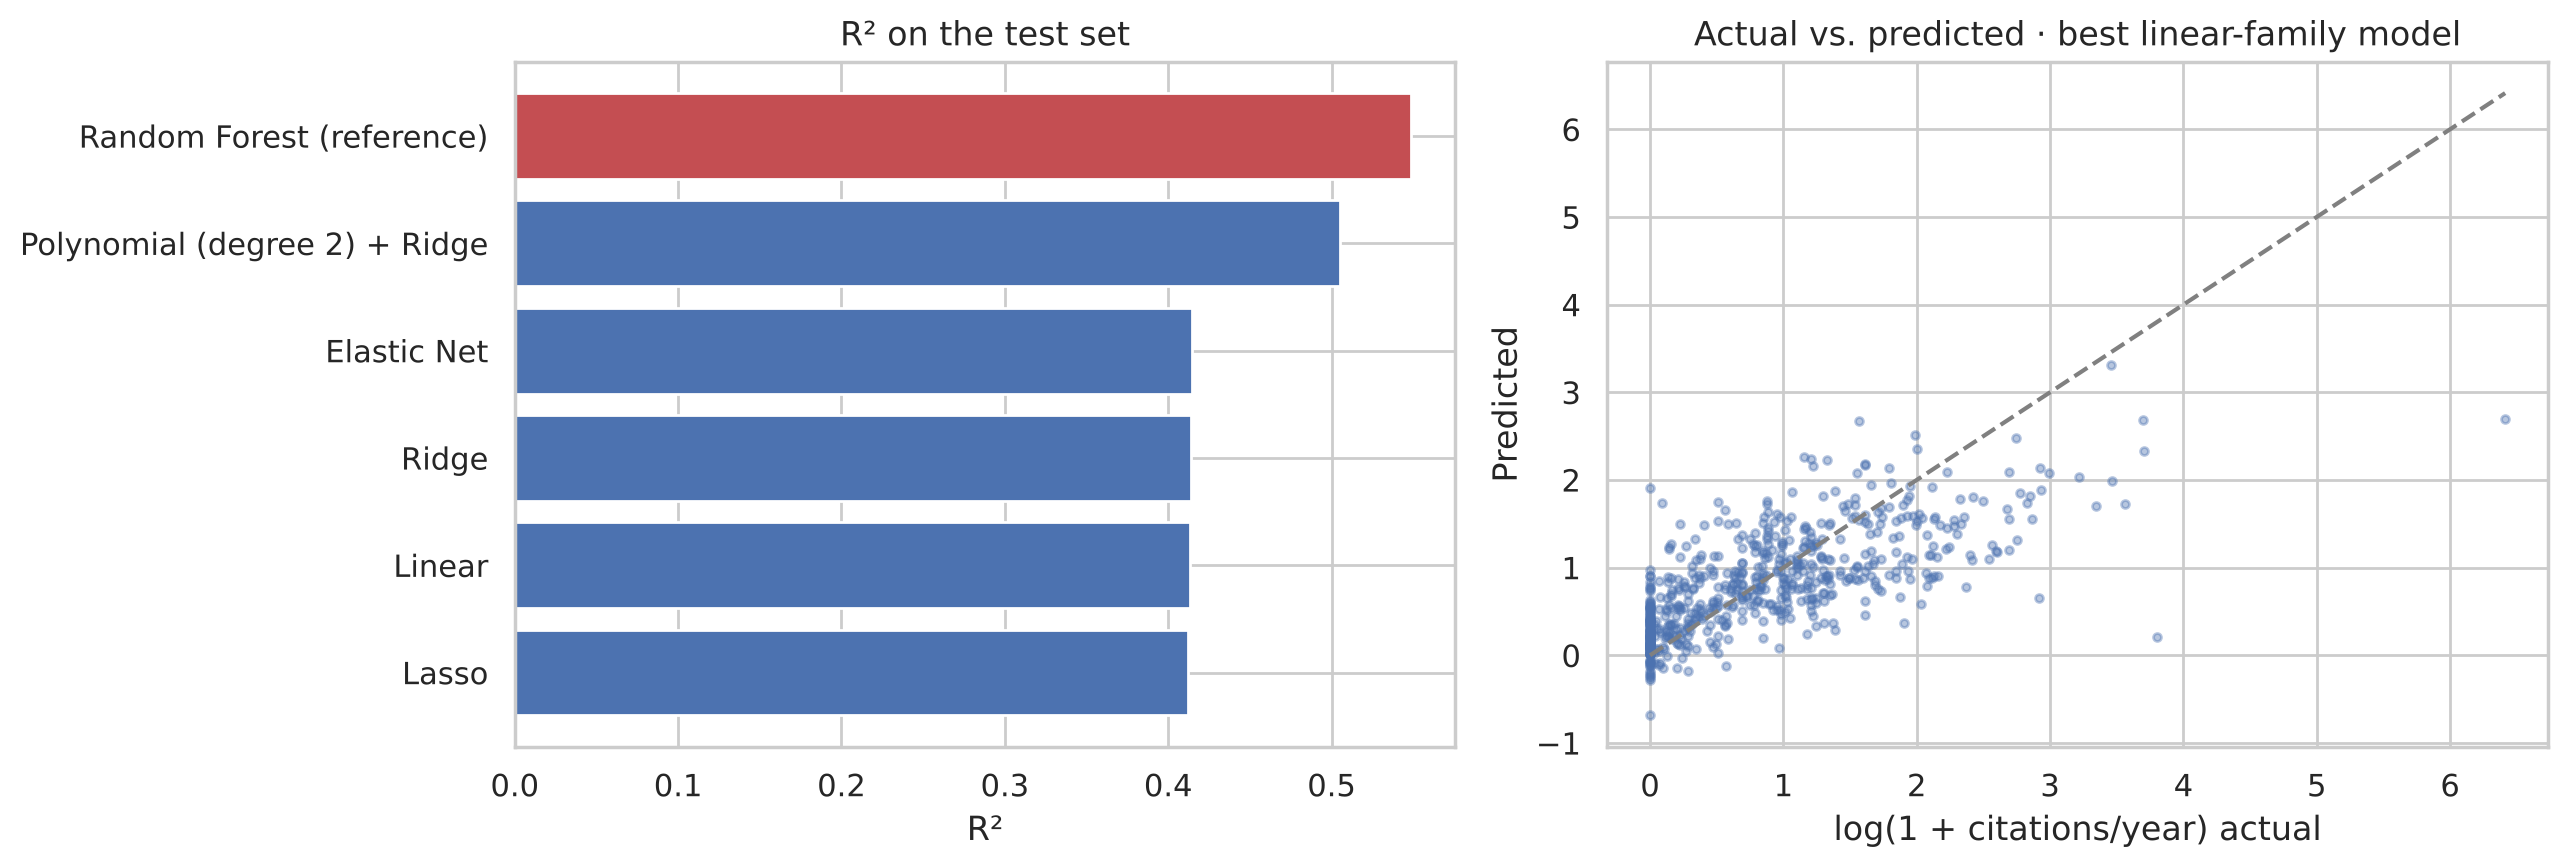
\includegraphics[width=\columnwidth]{reg_comparacion.png}
\caption{Comparison of regression models and actual versus predicted values.}
\label{fig:reg}
\end{figure}

\begin{figure}[t]
\centering
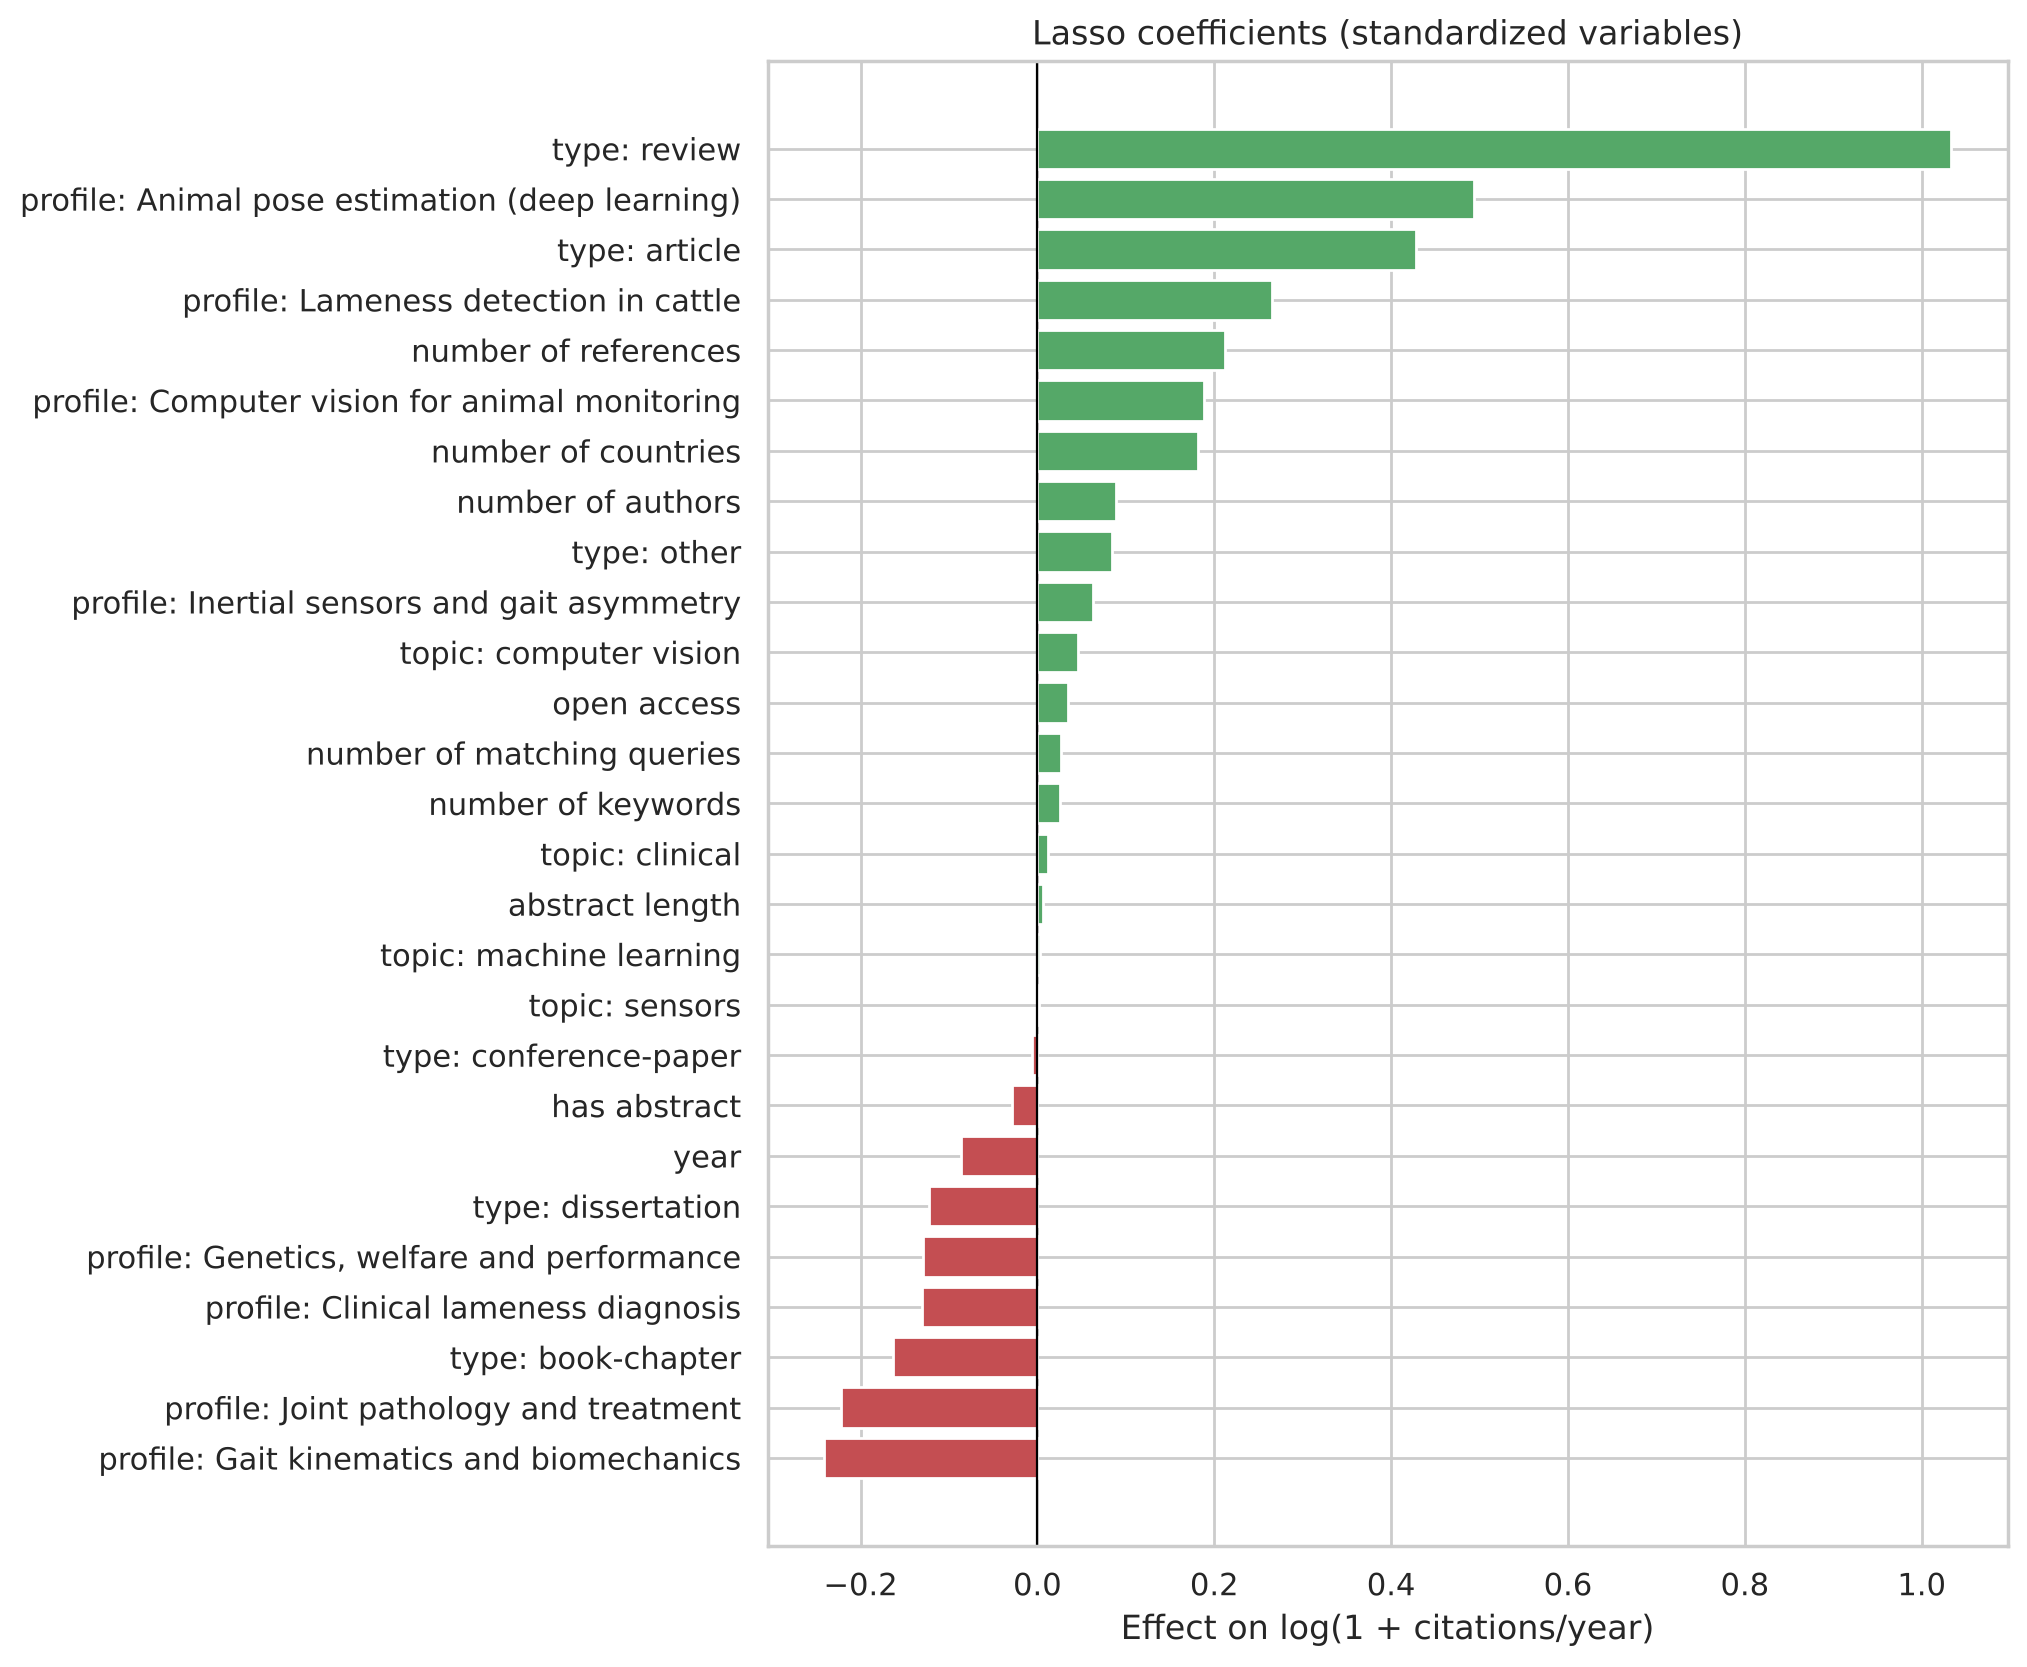
\includegraphics[width=0.9\columnwidth]{reg_lasso_coeficientes.png}
\caption{Lasso coefficients: characteristics associated with higher or lower impact of a paper.}
\label{fig:lasso}
\end{figure}

% =====================================================================
\section{Cost Analysis}
Costs were estimated with list prices for the us-east-1 region in two scenarios (Table~\ref{tab:costos}). The academic scenario matches the current use of the project, and the pilot projects fifty clinics running twenty thousand trot trials per month. The academic cost is practically zero thanks to the serverless design and to storing the key in Parameter Store, which is free, instead of Secrets Manager. In the pilot, storage is the main item, and the architecture scales without changes. The actual cost, checked in the AWS billing console, has been zero dollars since deployment, because the usage of these days was covered by the account's free tier. This is consistent with the estimate and confirms that the base system can run at no cost in an academic setting.

\begin{table}[t]
\centering
\caption{Estimated monthly cost in USD}
\label{tab:costos}
\begin{tabular}{lrr}
\toprule
Service & Academic & Pilot \\
\midrule
S3 and recovery replica & 0.17 & 9.80 \\
Lambda and API Gateway & 0.03 & 0.70 \\
DynamoDB and Athena & 0.03 & 1.46 \\
Parameter Store, ECR and CloudWatch & 0.15 & 1.55 \\
\midrule
\textbf{Total without free tier} & \textbf{0.38} & \textbf{13.51} \\
Total with free tier & 0.13 & 10.95 \\
\bottomrule
\end{tabular}
\end{table}

% =====================================================================
\section{Validation, Limitations and Future Work}
Validation relied on three practices: separation by horse throughout modelling, paired statistical tests at the animal level, and reproduction in the cloud of the local results. The main limitations are the small number of horses, the use of induced rather than natural lameness, and a single breed. Future work includes comparing each horse with its own baseline, identifying the side of the asymmetry, estimating the degree of lameness and, in the vision phase, computing these measures from video with a pose estimation model. In the longer term, the plan is to collect our own data from Colombian criollo horses assessed by veterinarians, whose gaits, such as the paso fino and the trocha, differ from the trot studied in the literature.

% =====================================================================
\section{Conclusions}
Data mining made it possible to map a field that is moving quickly towards computer vision and leaves a clear gap: there are no open data on equine video with lameness, and there is almost no Latin American research. The sensor data confirmed that the asymmetry of head and pelvis movement captures lameness in an interpretable way, and the model built on those measures works on horses it has never seen. The complete system, from ingestion to prediction, was deployed in the cloud as code, at almost no cost. If, in the next phase, computer vision estimates those same trajectories from a video, the model and infrastructure from this work are ready to receive them.

\section*{Ethics and Data}
Only public data with open licenses were used, and no personal data were processed. The experimental protocol of the sensor dataset is the responsibility of its authors. The system is a support tool and does not replace veterinary examination.

\begin{thebibliography}{99}
\bibitem{nehs2013} ``Equine health survey highlights the prevalence of lameness,'' \emph{Veterinary Record}, vol.~173, no.~6, p.~132, 2013, doi: 10.1136/vr.f4967.
\bibitem{usda1998} USDA APHIS, ``National economic cost of equine lameness, colic, and equine protozoal myeloencephalitis (EPM) in the United States,'' Info sheet, NAHMS Equine'98, Fort Collins, CO, USA.
\bibitem{keegan2010} K.~G. Keegan \emph{et al.}, ``Repeatability of subjective evaluation of lameness in horses,'' \emph{Equine Vet. J.}, vol.~42, no.~2, pp.~92--97, 2010, doi: 10.2746/042516409X479568.
\bibitem{hammarberg2016} M.~Hammarberg, A.~Egenvall, T.~Pfau, and M.~Rhodin, ``Rater agreement of visual lameness assessment in horses during lungeing,'' \emph{Equine Vet. J.}, vol.~48, no.~1, pp.~78--82, 2016, doi: 10.1111/evj.12385.
\bibitem{agronegocios2025censo} Agronegocios, ``¿Cuántos caballos hay en Colombia y de esta cifra cuántos están registrados?,'' 2025. [Online]. Available: \url{https://www.agronegocios.co/finca/cuantos-caballos-hay-en-colombia-y-de-esta-cifra-cuantos-estan-registrados-4206155}
\bibitem{un2015} United Nations, ``Transforming our world: the 2030 Agenda for Sustainable Development,'' Res. A/RES/70/1, 2015.
\bibitem{keegan2013} K.~G. Keegan \emph{et al.}, ``Comparison of a body-mounted inertial sensor system-based method with subjective evaluation for detection of lameness in horses,'' \emph{Am. J. Vet. Res.}, vol.~74, no.~1, pp.~17--24, 2013.
\bibitem{mathis2018} A.~Mathis \emph{et al.}, ``DeepLabCut: markerless pose estimation of user-defined body parts with deep learning,'' \emph{Nature Neuroscience}, vol.~21, pp.~1281--1289, 2018.
\bibitem{mathis2021} A.~Mathis \emph{et al.}, ``Pretraining boosts out-of-domain robustness for pose estimation,'' in \emph{Proc. IEEE/CVF WACV}, 2021, pp.~1859--1868.
\bibitem{li2024pferd} C.~Li \emph{et al.}, ``The Poses for Equine Research Dataset (PFERD),'' \emph{Scientific Data}, vol.~11, art.~497, 2024.
\bibitem{yu2021ap10k} H.~Yu \emph{et al.}, ``AP-10K: A benchmark for animal pose estimation in the wild,'' in \emph{NeurIPS Datasets and Benchmarks Track}, 2021.
\bibitem{yang2022apt36k} Y.~Yang \emph{et al.}, ``APT-36K: A large-scale benchmark for animal pose estimation and tracking,'' in \emph{NeurIPS Datasets and Benchmarks Track}, 2022.
\bibitem{ng2022animalkingdom} X.~L. Ng \emph{et al.}, ``Animal Kingdom: A large and diverse dataset for animal behavior understanding,'' in \emph{Proc. IEEE/CVF CVPR}, 2022, pp.~19023--19034.
\bibitem{ismail2024cow} S.~Ismail \emph{et al.}, ``CowScreeningDB: A public benchmark database for lameness detection in dairy cows,'' \emph{Comput. Electron. Agric.}, vol.~216, art.~108500, 2024.
\bibitem{wirth2000} R.~Wirth and J.~Hipp, ``CRISP-DM: Towards a standard process model for data mining,'' in \emph{Proc. 4th Int. Conf. Practical Applications of Knowledge Discovery and Data Mining}, 2000, pp.~29--39.
\bibitem{priem2022openalex} J.~Priem, H.~Piwowar, and R.~Orr, ``OpenAlex: A fully-open index of scholarly works, authors, venues, institutions, and concepts,'' arXiv:2205.01833, 2022.
\bibitem{smit2023dataset} I.~Smit \emph{et al.}, ``Kinematic data of the Icelandic horse with induced lameness at walk, trot and tölt,'' DataverseNL, 2025, doi: 10.34894/PEWAK6.
\bibitem{agrawal1994} R.~Agrawal and R.~Srikant, ``Fast algorithms for mining association rules,'' in \emph{Proc. 20th Int. Conf. Very Large Data Bases}, 1994, pp.~487--499.
\bibitem{han2000} J.~Han, J.~Pei, and Y.~Yin, ``Mining frequent patterns without candidate generation,'' in \emph{Proc. ACM SIGMOD}, 2000, pp.~1--12.
\bibitem{breiman2001} L.~Breiman, ``Random forests,'' \emph{Machine Learning}, vol.~45, no.~1, pp.~5--32, 2001.
\bibitem{lundberg2017} S.~M. Lundberg and S.-I. Lee, ``A unified approach to interpreting model predictions,'' in \emph{Advances in Neural Information Processing Systems 30}, 2017, pp.~4765--4774.
\bibitem{tibshirani1996} R.~Tibshirani, ``Regression shrinkage and selection via the lasso,'' \emph{J. Royal Statistical Society: Series B}, vol.~58, no.~1, pp.~267--288, 1996.
\bibitem{zou2005} H.~Zou and T.~Hastie, ``Regularization and variable selection via the elastic net,'' \emph{J. Royal Statistical Society: Series B}, vol.~67, no.~2, pp.~301--320, 2005.
\bibitem{terraform} HashiCorp, ``Terraform documentation,'' 2026. [Online]. Available: \url{https://developer.hashicorp.com/terraform/docs}
\end{thebibliography}

\end{document}
